\documentclass[12pt,draftcls,onecolumn]{IEEEtran}
%\documentclass[12pt,onecolumn]{IEEEtran}
\usepackage{times}
\usepackage{hyperref}
%!TEX root =  autocontgrlp.tex
\usepackage{etex}
\usepackage{multicol}
\setlength{\marginparwidth}{13mm}
\usepackage[textsize=tiny]{todonotes}
%\usepackage[disable]{todonotes}
\newcommand{\todoc}[2][]{\todo[color=red!20!white,#1]{Cs: #2}}
\newcommand{\todoch}[2][]{\todo[color=blue!20!white,#1]{C: #2}}
\newcommand{\todos}[2][]{\todo[inline,color=blue!20!white,#1]{S: #2}}
%\usepackage{enumitem}
%\usepackage[fleqn]{amsmath}
\usepackage{amsmath}
\usepackage{mathtools}
\usepackage{graphicx}
\usepackage{times}
\usepackage{helvet}
\usepackage{courier}
\usepackage{paralist}
\usepackage{latexsym}
\usepackage{url}
\usepackage[all]{xy}
\usepackage{amsmath}
\usepackage{amssymb}
\usepackage{amsthm}
\usepackage{nccmath} % mfrac
\usepackage{comment}
%\usepackage{enumitem}
\usepackage{paralist}
\usepackage{xcolor}
\usepackage[colorlinks=true,linkcolor=blue,citecolor=purple]{hyperref}
%\usepackage{hyperref}
\usepackage{graphicx}
\usepackage{pifont}
%\usepackage{algorithm}
%\usepackage{algorithmic}
%\usepackage{pseudocode}
%\usepackage{algpseudocode}
\usepackage{savesym}
\savesymbol{AND}
\usepackage{xspace}
\usepackage{tikz}
\usepackage{pgfplots}
\usepackage{pgf}
\usepackage{algorithm}
\usepackage{algorithmic}
\usepackage{xspace}
\usepackage{comment}
\usepackage{placeins}
\usepackage[capitalize]{cleveref}


%\usepackage{style/ssltr}
%\usepackage{style/macros}
\if0
\usetikzlibrary{intersections}
\usetikzlibrary{arrows,calc,fit,patterns,plotmarks,shapes.geometric,shapes.misc,shapes.symbols,   shapes.arrows,   shapes.callouts,   shapes.multipart,   shapes.gates.logic.US,   shapes.gates.logic.IEC,   er,   automata,   backgrounds,   chains,   topaths,   trees,   petri,   mindmap,   matrix,   calendar,   folding, fadings,   through,   positioning,   scopes,   decorations.fractals,   decorations.shapes,   decorations.text,   decorations.pathmorphing,   decorations.pathreplacing,   decorations.footprints,   decorations.markings, shadows,circuits}
\tikzstyle{decision}=[diamond,draw]
\tikzstyle{line}=[draw]
\tikzstyle{elli}=[draw,ellipse]
\tikzstyle{arrow} = [thick]
\fi
%\usepackage{subfig}
\newcommand{\ralp}{r_{\text{\sc ALP}}}
\newcommand{\Jalp}{J_{\text{\sc ALP}}}
\newcommand{\alp}{\text{\sc ALP}\xspace}
%\newcommand{\lralp}{\text{L\!R\!A\!L\!P}\xspace}
\newcommand{\lralp}{\text{\sc LRALP}\xspace}
\newcommand{\lralpshort}{\text{\sc LRA}\xspace}
\newcommand{\mb}{\mbox{ }}
\newcommand{\one}{\mathbf{1}}
\newcommand{\zero}{\mathbf{0}}
\newcommand{\nn}{\nonumber}
\newcommand{\minp}{(\min,+)}
\newcommand{\R}{\Re} %{\mathbb{R}}
\newcommand{\Rm}{\mathbf{R}_{\min}}
\newcommand{\ra}{\rightarrow}
\newcommand{\om}{\otimes}
\newcommand{\op}{\oplus}
\newcommand{\RA}{\Rightarrow}
\newcommand{\LA}{\Leftarrow}
\newcommand{\E}{\mathbb{E}}
\newcommand{\T}{\mathcal{T}}
\newcommand{\B}{\mathcal{B}}
\newcommand{\F}{\mathcal{F}}
\newcommand{\C}{\mathcal{C}}
\newcommand{\M}{\mathcal{M}}
\newcommand{\N}{\mathcal{N}}
\newcommand{\et}{||\Gamma J^*-\hg J^*||_\infty}
\newcommand{\etmn}{||\Gamma J^*-\hg J^*||_{\mn}}
\newcommand{\ini}{\lceil \frac{n}{k}\rceil}
\newcommand{\I}{\mathcal{I}}
\newcommand{\mut}{\tilde{\mu}}
\newcommand{\mn}{\infty,\psi}
\newcommand{\tj}{J_{\alp}} %{\tilde{J}}
\newcommand{\hj}{J_{\lralpshort}} %{\hat{J}}
\newcommand{\Jlr}{\hj}
\newcommand{\Jlralp}{\hj}
\newcommand{\jd}{J'}
\newcommand{\bj}{\bar{J}}
\newcommand{\tv}{V_{\alp}} %{\tilde{V}}
\newcommand{\hv}{V_{\lralpshort}} % {\hat{V}}

\newcommand{\Jalpo}{J^*_{\alp}}
\newcommand{\Jlro}{J^*_{\lralpshort}}
\newcommand{\rlr}{r_{\lralpshort}}

\newcommand{\tu}{\tilde{u}}
\newcommand{\hu}{\hat{u}}

\newcommand{\muh}{\hat{\mu}}
\newcommand{\mui}{{\mu}^i}

\newcommand{\br}{\bar{r}}
\newcommand{\hr}{r_{\lralpshort}} %{\hat{r}}
\newcommand{\har}{\hr} %{\hat{r}}
\newcommand{\tr}{r_{\alp}} %{\tilde{r}}
\DeclareMathOperator{\argmin}{argmin}
\DeclareMathOperator{\argmax}{argmax}
\newcommand{\norm}[1]{\|#1\|}
\newcommand{\inorm}[1]{\|#1\|_{\infty}}
\newcommand{\snorm}[1]{\left\|#1\right\|}
\newcommand{\sinorm}[1]{\left\|#1\right\|_{\infty}}


%\newcommand{\eqdef}{\stackrel{\text{\footnotesize def}}{=}}
%\newcommand{\eqdef}{\stackrel{\Delta}{=}}
\newcommand{\eqdef}{\doteq}
\newcommand{\defeq}{\doteq}

\newcommand{\eps}{\varepsilon}
\renewcommand{\epsilon}{\varepsilon}



\newcommand{\tg}{\tilde{\Gamma}}



\newcommand{\conf}{\sqrt{\frac{2\ln t}{t_i}}}
%\newcommand{\tg}{\tilde{\Gamma}}
\newcommand{\hg}{\hat{\Gamma}}
%\newcommand{\hg}{{\Gamma}_W}
\newcommand{\gd}{\Gamma'}
\newcommand{\vd}{V'}
%\newcommand{\qed}{\blacksquare}

\newcommand{\keywords}[1]{{\bf Keywords: } #1\par}
%\newenvironment{proof}{{\bf Proof:} }{}
\newtheorem{theorem}{Theorem}[section]
\newtheorem{lemma}[theorem]{Lemma}
\newtheorem{claim}[theorem]{Claim}
\newtheorem{proposition}[theorem]{Proposition}
\newtheorem{corollary}[theorem]{Corollary}
\newtheorem{assumption}{Assumption}[section]
\newtheorem{definition}{Definition}[section]
\newtheorem{remark}{Remark}[section]
\newtheorem{example}{Example}[section]
\newtheorem{note}{Note}[section]
\newcommand{\alert}[1]{\textcolor{red}{#1}} 
\newcommand{\J}{\mathcal{J}}


\def\v{\mathbf{v}}
\def\r{\mathbf{r}}
\def\p{\mathbf{p}}
\def\q{\mathbf{q}}
%\def\R{\mathrm{R}}
\def\Re{\mathbb{R}}
\def\Z{\mathbb{Z}}
\def\P{\mathrm{P}}
\def\S{\mathcal{S}}
\def\A{\mathcal{A}}

\newcommand{\ith}[2][th]{$#2^{\text{#1}}$}
\newcommand{\us}[2]{\underset{#2}{#1}~}
\newcounter{subequation}[equation]
\newcommand{\thesubequationonly}{\alph{subequation}}
\renewcommand{\thesubequation}{\text{\theequation(\thesubequationonly)}}
\newcommand{\subequationitem}{\refstepcounter{subequation}(\thesubequationonly)\thinspace}

\def\mathdisplay#1{%
  \ifmmode \@badmath
  \else
    $$\def\@currenvir{#1}%
    \let\dspbrk@context\z@
    \let\tag\tag@in@display \SK@equationtrue %\let\label\label@in@display
    \global\let\df@label\@empty \global\let\df@tag\@empty
    \global\tag@false
    \let\mathdisplay@push\mathdisplay@@push
    \let\mathdisplay@pop\mathdisplay@@pop
    \if@fleqn
      \edef\restore@hfuzz{\hfuzz\the\hfuzz\relax}%
      \hfuzz\maxdimen
      \setbox\z@\hbox to\displaywidth\bgroup
        \let\split@warning\relax \restore@hfuzz
        \everymath\@emptytoks \m@th $\displaystyle
    \fi
%   \fi
}

\newcommand{\algorithmicinput}{\textbf{Input:} }
\newcommand{\INPUT}{\item[\algorithmicinput]}
\newcommand{\algorithmicoutput}{\textbf{Output:} }
\newcommand{\OUTPUT}{\item[\algorithmicoutput]}
\newcounter{algostep}
\newcommand{\Step}[1][\STATE]{#1\textbf{\refstepcounter{algostep}\thealgostep}. }

\newenvironment{algoequation}{\refstepcounter{equation}$}{$\hfill (\theequation)}

\newenvironment{nonfloatalgorithm}[1]{\vspace{1ex}\hrule\vspace{0.5ex} \refstepcounter{algorithm}\textbf{Algorithm \thealgorithm}\hspace{1em} #1 \vspace{0.5ex}\hrule}{\hrule\vspace{1.5ex}\setcounter{algostep}{0}}

\newcounter{acalgorithm}

\newenvironment{nonfloatactorcriticalgorithm}[1]{\vspace{1ex}\hrule\vspace{0.5ex} \textbf{Actor-Critic Algorithm \refstepcounter{acalgorithm}\theacalgorithm}\hspace{1em} #1 \vspace{0.5ex}\hrule\addcontentsline{loa}{algorithm}{\protect\numberline{\theacalgorithm}{\ignorespaces #1}}}{\hrule\vspace{1.5ex}\setcounter{algostep}{0}}

%\documentstyle[nips14submit_09,times,art10]{article} % For LaTeX 2.09
\title{A Generalized Reduced Linear Program for Markov Decision Processes}
\author{Chandrashekar Lakshminarayanan and Shalabh Bhatnagar\\Department of Computer Science and Automation\\ Indian Institute of Science\\ Bangalore-560012\\\{chandrul,shalabh\}@csa.iisc.ernet.in\\ and \\
Csaba Szepesv\'{a}ri\\Department of Computing Science\\University of Alberta\\Edmonton, Alberta\\Canada T6G 2E8\\  csaba.szepesvari@ualberta.ca }

% The \author macro works with any number of authors. There are two commands
% used to separate the names and addresses of multiple authors: \And and \AND.
%
% Using \And between authors leaves it to \LaTeX{} to determine where to break
% the lines. Using \AND forces a linebreak at that point. So, if \LaTeX{}
% puts 3 of 4 authors names on the first line, and the last on the second
% line, try using \AND instead of \And before the third author name.
\newcommand{\fix}{\marginpar{FIX}}
\newcommand{\new}{\marginpar{NEW}}
%\nipsfinalcopy % Uncomment for camera-ready version
\begin{document}
\maketitle
%!TEX root =  autocontgrlp.tex
\begin{abstract}
Approximate linear programming (ALP) and its variants have been widely applied to Markov Decision Processes (MDPs) with a large number of states. A serious limitation of ALP is that it has an intractable number of constraints, as a result of which constraint approximations are of interest. In this paper, we define a generalized reduced linear program (GRLP) that has a tractable number of constraints, which are obtained as positive linear combinations of the original constraints of the ALP. The main contribution of this paper is a novel theoretical framework developed to obtain error bounds for any given GRLP. By providing a detailed error analysis for the GRLP, we justify usage of a linear architecture for approximating the dual variables. Unlike prior results on constraint sampling, our analysis is deterministic and is based on a novel contraction operator.
\end{abstract}
\begin{keywords}{
Approximate Dynamic Programming (ADP), Markov Decision Processes (MDPs), Approximate Linear Programming (ALP), Generalized Reduced Linear Program (GRLP), Constraint Sampling, Reinforcement Learning.}
\end{keywords}

%!TEX root =  autocontgrlp.tex
\section{Introduction}
Markov decision processes (MDPs) are a powerful mathematical framework to study optimal sequential decision making problems  arising in science and engineering. In an MDP, the configuration of the system is described by the state variables (or simply the state) and the system evolves in a stochastic manner which depends on the action made. The set of all states is denoted by $S$, the state space and the set of all actions is denoted by $A$, the action space.
%An instance of an MDP is a controlled queue setting, where there is a cost associated with the number of customers in the queue, and the aim is to control the service level depending on the number of %customers so as to achieve a minimum cumulative cost. In more general terms, given any MDP,
We are interested in computing what is known as the optimal policy $u^*$ (a map from $S$ to $A$). The so-called dynamic programming (DP) methods first compute what is known as the optimal \emph{value-function} ($J^*$), a vector whose dimension is the number of states, and use it to compute $u^*$. When the number of state is small conventional DP techniques, such as value-, or policy-iteration, or linear programming (LP) can be used to compute $J^*$ and $u^*$\cite{BertB}.\par
As the number of states is grows, it becomes increasingly difficult to compute the exact values of $J^*$ and $u^*$. A practical solution then is to compute an approximate value function $\tilde{J}$ instead of $J^*$. Approximate dynamic programming (ADP) methods combine an approximation architecture to represent $\tj$ and a conventional DP method to compute $\tj$. Eventually, ADP methods output a sub-optimal policy $\tu$ using the $\tj$ they compute. %Here, success depends on the quality of approximation, i.e., on the quantity $||J^*-\tilde{J}||$ for an appropriately chosen norm.\par
Linear function approximation (LFA), i.e., letting $\tilde{J}=\Phi r^*$ where $\Phi$ is a so-called feature matrix and $r^*$ is a weight vector to be computed, is the most widely used method of approximation. Here, dimensionality reduction is achieved by choosing $\Phi$ to have fewer columns in comparison to the number of states, holding the promise of being able to work with MDPs regardless of the number of states.\par
It is natural to expect that approximations lead to errors and it is important to quantify the errors. For a given ADP method, theoretical performance analysis analytically bounding the error terms $||J^*-\tilde{J}||$  and $\norm{J^*-J_{\tu}}$ which denote the error in approximating the value function, and performance loss due to following policy $\tu$ (here $J_{\tu}$ is the value of $\tu$) respectively. Further, in most cases the error terms reveal some structure that can offer insights and act as guide to the designer of the ADP method (for example the choice of $\Phi$). \par

%While many ADP methods use LFA, not all of them are successful. For instance, ADP methods that use linear least squares projection are known to exhibit `policy oscillations' \cite{dpchapter}, i.e., %output a repeating sequence of bad sub-optimal policies.
%Such an analysis is important to establish that the error is always bounded.
%Further, in most cases the error terms reveal some structure that can offer insights and act as guide to the designer of the ADP method (for example the choice of $\Phi$). \par

The \emph{approximate linear program} (ALP) \cite{ALP,CS,SALP,ALP-Bor} and its variants combine LFA and the LP approach. Theoretical performance analysis of the ALP can be found in \cite{ALP}.
%and a salient feature is that it does not suffer from issues such as `policy oscillations'\footnote{ADP methods that use linear least squares projection are known to exhibit `policy oscillations' %\cite{BertB}, i.e., output a repeating sequence of bad sub-optimal policies. Since our focus in this paper is the ALP formulation, we refrain from a detailed presentation of the other methods.}

A critical shortcoming of vanilla ALP is that the number of constraints are of the order of the size of the state space, making this vanilla version intractable. Two approaches have been found empircally successful in addressing the issue of large number of constraints in the ALP. In the first approach, a random subset of constraints is chosen (dropping the rest), thereby formulating a \emph{reduced linear program} (RLP). The performance analysis of the RLP can be found in \cite{CS}, however, the bounds hold only in high probability under idealized assumptions. The second approach involves employing function approximation in the dual variables of the ALP \cite{ALP-Bor,dolgov}. However, to this date, there exist no theoretical guarantees bounding the loss in performance due to this approach.\par
Our motivation stems from the fact that ALP with tractable number of constraints will result in a full dimeniosnality free ADP method. However, constraint reduction in the ALP is an extra source of error (in addition to the error due to LFA), which has not been theoretically well understood.  The focus of this paper is to fill this gap in theory by deriving performance bounds for constraint reduction in the ALP formulation.
The salient aspects of our contribution are listed below:
\begin{enumerate}
\item We define a generalized reduced linear program (GRLP) which has a tractable number of constraints that are obtained as positive linear combinations of the original constraints. The GRLP amounts to linear function approximation of the dual variables, and the RLP is a special case of GRLP.
		\item We develop novel analytical machinery to relate $\hat{J}$, the solution to the GRLP, and the optimal value function $J^*$ by bounding the prediction error $||J^*-\hj||$ (\Cref{cmt2mn}). 
		\item We also bound the performance loss due to using the policy $\hu$ that is one-step greedy with respect to $\hj$ (Theorem~\ref{polthe}).
		\item Our analysis is based on two novel $\max$-norm contraction operators and our results hold \emph{deterministically}, as opposed to the results on RLP \cite{SALP,CS}, where the guarantees have a probabilistic nature.
%Our analysis also makes use of arguments based on \emph{Lyanpunov} function, an approach much similar to prior works in ALP literature \cite{ALP,SALP}.
\item Our results on the GRLP are the first to theoretically analyze the use of linear function approximation of Langrangian (dual) variables underlying the constraints.
\item A numerical example in controlled queues is provided to illustrate the theory.
\end{enumerate}
%ALP with tractable number of constraints would result in  a full dimensionality free ADP method, without issues such as policy oscillations.
A short and preliminary version of this paper without the theoretical analysis is available in \cite{aaaipaper}.

%!TEX root =  autocontgrlp.tex
\section{Markov Decision Processes (MDPs)}
In this section, we briefly discuss the basics of Markov Decision Processes (MDPs) (the reader is referred to \cite{BertB,Puter} for a detailed treatment).\\
An MDP is a $4$-tuple $\langle S,A,P,g\rangle$, where $S$ is the state space, $A$ is the action space, $P$ is the probability transition kernel and $g$ is the reward function. We consider MDPs with large but finite number of states. We also assume that the number of actions is finite.
Without the loss of generality, we set  $S=\{1,2,\ldots,n\}$  and the action set is given by $A=\{1,2,\ldots,d\}$. For simplicity, we assume that all actions are feasible in all states. The probability transition kernel $P$ specifies the probability $p_a(s,s')$ of transitioning from state $s$ to state $s'$ under the action $a$. We denote the reward obtained for performing action $a\in A$ in state $s\in S$ by $g_a(s)$.

A policy $\mu$ specifies the action selection mechanism, and is described by the sequence $\mu=(u_1,u_2,\ldots,u_n,\ldots)$, where $u_n\colon S \ra A$ for all $n \geq 0$. \todoc{This is somewhat limited; normally we should allow history dependent,
and also stochastic policies.} 
A stationary deterministic policy (SDP) is one where $u_n\equiv u$ for all $n\geq 0$ for some $u\colon S \ra A$. By abuse of notation we denote the SDP by $u$ itself instead of $\mu$. In the setting that we consider, one can find an SDP that is optimal \cite{BertB,Puter}. In this paper, we restrict our focus to the class $U$ of SDPs.  Under an SDP $u$, the MDP is a Markov chain with probability transition kernel $P_u$.

Given an SDP $u$, the infinite horizon discounted reward corresponding to state $s$ under $u$ is denoted by $J_u(s)$ and is defined by
\begin{align}
J_u(s)\stackrel{\Delta}{=}\E[\sum_{n=0}^\infty \alpha^n g_{a_n}(s_n)|s_0=s,a_n=u(s_n), n= 0,1,\dots],\nn
\end{align}
where $\alpha \in (0,1)$ is a given discount factor. Here $J_u(s)$ is known as the value of the state $s$ under the SDP $u$, and the vector quantity $J_u\stackrel{\Delta}{=}(J_u(s))_{s\in S}\in R^n$ is called the value-function corresponding to the SDP $u$.\\
The optimal policy $u^*$ is any policy whose value is the largest possible under any policy: 
$J_{u^*}(s) = \max_{u\in U} J_u(s)$ for all $s\in S$. Such $u^*$ exists and is well defined in the case of infinite horizon discounted reward MDP \cite{Puter}.
\todoc{A stronger definition allows any policy, including history dependent and yet the statement will hold true.}
 The optimal value-function $J^*$ is the one obtained under the optimal policy, i.e., $J^*=J_{u^*}$. \todoc{Probably better to define first $J^*$ as the pointwise max and then the optimal policy's definition could use $J^*$.}
Given an MDP, our aim is to find the optimal value function $J^*$ and the optimal policy $u^*$. The optimal policy and value function obey the Bellman equation (BE): for all $ s \in S$, \todoc{Non-unique maximizers in the policy def?}
\begin{subequations}\label{bell}
\begin{align}
\label{bellval}J^*(s)&=\max_{ a\in A}\big(g_a(s)+\alpha \sum_{s'}p_a(s,s')J^*(s')\big),\\
\label{bellpol}u^*(s)&=\arg\max_{ a\in A}\big(g_a(s)+\alpha \sum_{s'}p_a(s,s')J^*(s')\big).
\end{align}
\end{subequations}
If $J^*$ is computed first, then $u^*$ can be obtained by substituting $J^*$ in \eqref{bellpol}. The Bellman operator $T$ is defined using the model parameters of the MDP as follows:
\begin{definition}
The Bellman operator $T: \R^n \to \R^n$ is defined by 
\begin{align}
(TJ)(s)=\max_{a \in A}\big(g_a(s)+\alpha \sum_{s'} p_a(s,s')J(s')\big)\,, 
\end{align}
where $J\in \R^n$ and $J_s = J(s)$, $s\in S = \{1,\dots,n\}$.  
Similarly one can define the Bellman operator $T_u:\R^n \to \R^n$ restricted to an SDP $u$ as follows:
\begin{align}
(T_uJ)(s)=g_{u(s)}(s)+\alpha \sum_{s'} p_{u(s)}(s,s')J(s')\,.
\end{align}
\end{definition}
Given $J \in \R^n$, $TJ$ is the `one-step' greedy value function. It is also useful to define the notion of a one-step greedy policy as below:
\begin{definition}
A policy $\tilde{u}$ is said to be greedy with respect to $\tilde{J}$ if
\begin{align}\label{subpol}
\tilde{u}(s)=\underset{a \in A}{\argmax} \, \big(g_a(s)+\alpha\sum_{s'} p_a(s,s')\tilde{J}(s')\big)\,.
\end{align}
\end{definition}
We also define the Bellman operator $H$ for action values  \cite{BertB}: \todoc{$Q$-Bellman is a bad name.}
\begin{definition}
Let $H: \R^n \to \R^{nd}$ be defined as follows: For $J\in \R^n$,
\begin{align}
HJ&=\left[ {\begin{array}{c} H_1 J  \\ \vdots \\ H_d J\end{array}} \right]\in \R^{nd},\mbox{where}\nn\\
(H_a J)(s)&= g_a(s)+\alpha \sum_{s'}p_a(s,s') J(s'), \qquad s\in S, a\in A.
\end{align}
\end{definition}
 We now state without proof the important properties related to the Bellman operator. Though in these results, we make use of the Bellman operator $T$, the results also trivially hold for $T_u$ as well.
\subsection{Properties of $T$}
\begin{lemma}\label{maxnorm}
$T$ is a $\max$-norm contraction operator, i.e., given $J_1, J_2 \in \mathbf{R}^n$,
\begin{align}
||TJ_1-TJ_2||_\infty\leq \alpha ||J_1-J_2||_\infty.
\end{align}
\end{lemma}
\begin{corollary}\label{uniquesol}
$J^*$ is a unique fixed point of $T$, i.e., $J^*=TJ^*$.
\end{corollary}
The Bellman operator $T$ exhibits two more important properties presented in the following lemmas (see \cite{BertB} for proofs):
\begin{lemma}\label{monotone}
$T$ is a monotone map, i.e., given $J_1,J_2 \in \R^n$ such that $J_2\geq J_1$, we have $T J_2\geq T J_1$. Further, if $J\in \R^n$ is such that $J\geq TJ$, it follows that $J\geq J^*$.
\end{lemma}
\begin{lemma}\label{shift}
Given $J\in \R^n$, $t \in \R$ and $\mathbf{1} \in \R^n$, a vector with all entries $1$, we have
\begin{align}
T(J+t\mathbf{1})=TJ+\alpha t\mathbf{1}.
\end{align}
\end{lemma}
Note that Lemmas~\ref{maxnorm}-\ref{shift} also hold for the $Q$-Bellman operator $H$.
Solving an MDP involves handling two sub-problems namely the problem of \emph{control} and the problem of \emph{prediction}. The problem of \emph{control} deals with coming up with a good (and if possible the optimal) policy. Often, in order to solve the problem of \emph{control}, one needs to solve the problem of \emph{prediction}, which deals with computing the value function $J_u$ of the policy $u$. The fact that the two problems are related is reflected in the Bellman equation in \eqref{bell}, where $J^*$ from \eqref{bellval} is used in \eqref{bellpol} to obtain the optimal policy $u^*$. Thus, the Bellman equation is at the heart of the solution methods to MDPs. Any solution method to MDP is said to be complete only if it satisfactorily (with provable performance guarantees) addresses both the prediction and the control problems. \\
The basic solution methods namely value iteration, policy iteration and linear programming (LP) formulation \cite{BertB} solve both the control and prediction problems. Of the three basic methods, in this paper, we are interested in the LP formulation given by
\begin{align}\label{mdplp}
\begin{split}
\min_{J\in \R^n}\, &c^\top J\\
\text{s.t}\mb &J(s)\geq g_a(s)+\alpha\sum_{s'}p_a(s,s')J(s'), \qquad s\in S, a \in A,
\end{split}
\end{align}
where $c\in \R^n_+$ is any vector whose components are all non-negative. One can show that $J^*$ is the solution to the LP formulation \eqref{mdplp} \cite{BertB}. 
Also, of the three methods, value iteration and LP formulation are value function based methods, i.e., they compute $J^*$ directly and then $u^*$ is obtained by plugging $J^*$ in \eqref{bellpol}.\\
While the basic methods (i.e., VI, PI and LP) can be used to compute exact values $J^*$ and $u^*$ for MDPs with a small number of states, they are computationally expensive in the case of MDPs with a large number of states.\\

%!TEX root =  autocontgrlp.tex
\section{Approximate Dynamic Programming}
\emph{Curse-of-dimensionality} is a term used to denote the fact that the number of states and computational costs grow exponentially in the dimensions of the state space. \todoc{This itself won't be a curse, would it be? The problem is that the computation cost also grows exponentially. Note that we never defined what we mean by state variables.}
Most MDPs arising in practical applications suffer from the curse, i.e., have large number of states and it is difficult to compute $J^*/J_u\in \R^n$ exactly in such scenarios. Approximate dynamic programming (ADP) \cite{lspi,lspe,ALP,wang2014approximate} methods compute an approximate value function $\tilde{J}$ instead of $J^*/J_u$. In order to tackle the curse, ADP methods resort to dimensionality reduction by parametrizing the value function and/or the policy. Value-function based ADP methods form an important subclass of ADP methods whose brief overview is given below.

\subsection{Value-Function based ADP}
In the value-function based ADP schemes a parametrized family is chosen and the approximate value-function $\tilde{J}$ is picked from the chosen parametrized class.
Once the approximate value function $\tilde{J}$ is computed, a sub-optimal policy $\tilde{u}$ can be obtained as the one-step greedy policy with respect to $\tilde{J}$ by making use of \eqref{subpol}.
The following lemma characterizes the degree of sub-optimality of the greedy policy $\tilde{u}$.
\begin{lemma}\label{subopt}
Let $\tilde{J}$ be the approximate value function and $\tilde{u}$ be as in \eqref{subpol}, then 
\begin{align}
||J^*-J_{\tilde{u}}||_\infty \leq \frac{2}{1-\alpha}||J^*-\tilde{J}||_\infty\,.
\end{align}
\end{lemma}
The quality of any ADP method depends on the approximation guarantees it offers for the quantities $||J^*-\tilde{J}||$ and $||J^*-J_{\tu}||$, where $||\cdot||$ is an appropriate norm. The term  $||J^*-\tilde{J}||$ denotes the error in prediction and $||J^*-J_{\tu}||$ denotes the loss in performance resulting from the sub-optimal policy $\tu$ with respect to the optimal policy $u^*$. Of the two error terms, $||J^*-J_{\tu}||$ is more important because ultimately we are interested in coming up with a useful policy. In the context of ADP methods, the control and prediction problems are said to be addressed when the error terms $||J^*-\tilde{J}||$ and $||J^*-J_{\tu}||$ are bounded by ``small'' constants.

\subsection{Linear Function Approximation}
The most widely used parametrized class to approximate the value-function is the linear function approximator (LFA). Under LFA, the value-function is approximated as $\tilde{J}=\Phi r^*$, with $\Phi=[\phi_1|\ldots|\phi_k]$ being an $n\times k$ feature matrix and $r^*$ is the parameter to be learnt.

There are two important approaches to value function approximation. Both the approaches start out with a basic solution method and appropriately introduce function approximation in it. The two approaches are:
\begin{enumerate}
\item The Projected Bellman Equation (PBE) which combines the BE and the linear least squares projection operator to project high dimensional quantities onto the subspace of the LFA.
\item The approximate linear programming formulation which introduces the LFA in the linear programming formulation. 
\end{enumerate}
A host of ADP methods are based on the PBE and have been found to be useful in practice. The main application of the PBE is for approximate policy evaluation, i.e., to compute $\tilde{J}_u$, an approximation to the value function $J_u$ of policy $u$. Due to the mismatch in the norms, i.e, the linear least squares projection operator based on the $L_2$-norm and the $L_\infty$-norm of the Bellman operator $T$, one cannot use the PBE to obtain a direct approximation to $J^*$. Thus in order to solve the problem of control, $\tilde{J}_u$ is used to compute a one-step greedy policy. However, again due to the mismatch in the norms, i.e., $L_2$-norm of the linear least squares projection and the $L_\infty$ norm required for policy improvement (Lemma~\ref{subopt}), the one-step greedy policy need not necessarily be an improvement. This leads to a phenomenon called \emph{policy-chattering} \cite{dpchapter} where looping within of bad policies can occur. Further, such policy-chattering can be demonstrated in simple examples as well \cite{dpchapter}. Thus, though the approximate value function obtained by solving the PBE offers guarantees for prediction it does not offer any guarantees for the control problem, a significant shortcoming of the PBE based methods.

The ALP formulation \cite{ALP} on the other hand does not suffer from issues such as policy-chattering, for the simple reason that it computes $\tilde{J}$ which is an approximation to $J^*$ and a one-step greedy policy $\tilde{u}$ obtained using $\tilde{J}$. In short, since there is only one policy that the ALP outputs there is no question of policy-chattering. Further, the ALP offers performance guarantees for both the error terms $||J^*-\tilde{J}||$ and $||J^*-J_{\tilde{u}}||$. Though the ALP is a complete method addressing both the control and prediction problems, it nevertheless suffers from an important limitation in the form of large number of constraints (as large as the size of the state space). This limitation has been addressed in literature by sampling only a fewer tractable constraints to formulate a reduced linear program (RLP). The RLP has been shown to perform well in practice \cite{ALP,CS,CST}, but theoretical performance guarantees \cite{CS} are available for a specific RLP obtained under idealized assumptions. In this paper, by providing a sound theoretical analysis of the RLP, we aim to show that RLP is a complete method that addresses both the prediction and the control problems.
We achieve this by developing and presenting a comprehensive theoretical framework to understand the constraint reduction/approximation procedure.

In the next section, we discuss the approximate linear programming (ALP) formulation, the basic results and present prior results in literature as well as motivate the problem that we address in this paper. 

%!TEX root =  autocontgrlp.tex
\section{Approximate Linear Programming}
The LP formulation in \eqref{mdplp} can be represented in short as,
\begin{align}\label{mdplpshort}
\min_{J\in \R^n} &c^\top J\nn\\
\text{s.t}\mb &J\geq T J,\\
\textbf{or}\nn\\
\label{shortalter}
\min_{J\in \R^n} &c^\top J\nn\\
\text{s.t}\mb &EJ\geq H J,\\
\end{align}
where $J\geq TJ$ is a shorthand for the $nd$ constraints in \eqref{mdplp} and $E$ is an $nd\times n$ matrix given by $E=[I,\ldots,I]^\top$, i.e., $E$ is obtained by stacking $d$ identical $n\times n$ identity matrices one over the other. Note that \eqref{mdplpshort} and \eqref{shortalter} are identical programs and differ only in notation. We use notation of type \eqref{mdplpshort} whenever we prefer brevity and we use notation \eqref{shortalter} in some definitions and proof for the sake of clarity.
The approximate linear program (ALP) is obtained by making use of LFA in the LP, i.e., by letting $J=\Phi r$ in \eqref{mdplpshort} and is given as
\begin{align}\label{alp}
\min_{r\in \R^k} &c^\top \Phi r\nn\\
\text{s.t}\mb &\Phi r\geq T \Phi r.
\end{align}
Unless specified otherwise we use $\tr$ to denote the solution to the ALP and $\tj=\Phi \tr$ to denote the corresponding approximate value function. We now state the assumptions and definitions used for the rest of the paper.
\begin{assumption}\label{one}
The first column of the feature matrix $\Phi$ (i.e., $\phi_1$) is $\one \in \R^n$. In other words, the constant function is part of the basis.
\end{assumption}
\begin{assumption}\label{probdist}
$c=(c(i),i=1,\ldots,n)\in \R^n$ is a probability distribution, i.e., $c(i)\geq 0$ and $\sum_{i=1}^n c(i)=1$.
\end{assumption}
\begin{definition}
Given a function $\chi\colon S\ra \R^+$ we define the quantity $\beta_{\chi}$ as
\begin{align}
\beta_{\chi}=\max_{s \in S} \frac{\underset{a \in A}{\max}\big(\alpha\sum_{s'}p_a(s,s')\chi(s')\big)}{\chi(s)}.
\end{align}
\end{definition}
\begin{definition}
The function $\chi$ is then said to be a \emph{Lyapunov} function if $\beta_{\chi}<1$.
\end{definition}
\begin{assumption}\label{lyap}
$\psi\colon S \ra \R^+$ is a Lyapunov function and is present in the column span of the feature matrix $\Phi$.
\end{assumption}
It is straightforward to check that the function $\one$ is a Lyapunov function and trivially is present in the column span of $\Phi$. 
\begin{definition}\label{modlone}
The modified $L_1$-norm is defined as \todoc{modified $\Rightarrow$ weighted?}
\begin{align}
||J||_{1,c}=\sum_{s \in S} c(s)|J(s)|,
\end{align}
where $c$ obeys Assumption~\ref{probdist}.
\end{definition}
\begin{definition}\label{modnorm}
The modified $L_\infty$-norm is defined as follows:  \todoc{modified $\Rightarrow$ weighted? Also, the convention in math is to divide in the case of the $L_{\infty}$ norm. Not a high priority to change this, but maybe it would be good to do this in the longer term.}
\begin{align}
||J||_{\infty,\rho}=\max_{s \in S} \rho(s) |J(s)|,
\end{align}
where $\rho \colon \S \ra \R^+$, $J\in \R^n$.
\end{definition}
In Definition~\ref{modnorm}, the use of the weighting function $\rho$ allows us to measure the error taking into account the relative importance of the various states. A lower value of $\rho(s)$ means that the state $s$ is less important and vice-versa.\\
We recall below Theorem~$4.2$ of \cite{ALP} which bounds the error in the approximate value function.
\begin{theorem}\label{restateval}
Let $\tr$ be the solution to the ALP in \eqref{alp}, $\tilde{J}_c=\Phi \tilde{r}_c$, $\psi$ be a Lyapunov function and $c$ be a distribution as in \eqref{probdist}, then 
\begin{align}
||J^*-\tj||_{1,c}\leq \frac{2c^\top \psi}{1-\beta_{\psi}}\min_{r}||J^*-\Phi r||_{\mn}.
\end{align}
\end{theorem}
We now recall Theorem~$3.1$ of \cite{ALP} that characterizes the loss in performance of the greedy policy.
\begin{theorem}\label{restatepol}
Let $\tilde{u}$ be the greedy policy with respect to the solution $\tj$ of the ALP, then 
\begin{align}
||J^*-J_{\tu}||_{1,c}\leq \frac{1}{1-\alpha}||J^*-\tj||_{1,c'},
\end{align}
where $c'=(1-\alpha)c^\top(I-\alpha P_{\tu})^{-1}$.
\end{theorem}
Theorems~\ref{restateval} and ~\ref{restatepol} together imply that the ALP addresses both the control and prediction problems. Please refer to \cite{ALP} for a more detailed treatment of the ALP.\\
Note that the ALP is a linear program in $k$ ($<<n$) variables as opposed to the LP in \eqref{mdplpshort} which has $n$ variables. Nevertheless, the ALP has $nd$ constraints (same as the LP) which is an issue when $n$ is large and calls for constraint approximation/reduction techniques.

\section{Constraint sampling}
The most important work in the direction of constraint reduction is constraint sampling \cite{CS} wherein a reduced linear program (RLP) is solved instead of the ALP. While the objective function of the RLP is the same as that of the ALP, the RLP has only $m<<nd$ constraints sampled from the original ALP according to a given probability distribution. The reduced linear program is then given by
\small
\begin{align}\label{rlp}
\min_{J\in \R^n} &c^\top J\nn\\
\text{s.t}\mb &J(s)\geq g_a(s)+\alpha\sum_{s'}p_a(s,s')J(s'), \mb\forall (s,a) \in \I,
\end{align}
\normalsize
where $\I$ is the index set containing the $m$ sampled state-action pairs. Using the index set $\I$ we define an $nd\times m$ matrix $\M$, called the constraint sampling matrix as below.
\begin{definition}\label{csampmat}
Let $\I=\{(s_1,a_1),\ldots,(s_m,a_m)\}$ be the sampled state-action pairs and let $q_i\stackrel{\Delta}{=}s_i+(a_i-1)\times n,\forall i=1,\ldots,m$. Then the constraint sampling matrix associated with the index set $\I$ is given by
\begin{align}
\M(i,j)&=1, \mb\text{if}\mb q_i=j\nn\\
&=0, \mb\text{otherwise}.
\end{align}
\end{definition}
The RLP can then be represented in short as
\begin{align}\label{rlpshort}
\min_{r\in \N} &c^\top \Phi r\nn\\
\text{s.t}\mb & \M^\top E \Phi r \geq \M^\top H \Phi r,
\end{align}
where $\M$ is a constraint sampling matrix as in Definition~\ref{csampmat} and $\N\subset \R^k$ is a bounded set such that $\tr \in \N$. Note that the feasible set of the RLP is a superset of the feasible set of the ALP.\\
The RLP based on constraint sampling has been found to perform well empirically in application domains ranging from controlled queuing networks (see section $6.2$ of \cite{ALP} and section $7$ of \cite{SALP}) to Tetris (see \cite{CST} and section $6$ of \cite{SALP}). However, the theoretical guarantees for the RLP are available only under a restricted setting \cite{CS}. We present the main result of \cite{CS} on constraint sampling, and to that end define the following:
\begin{definition}\label{sampdist}
Given a policy $u$ and Lyapunov function $\psi$ in the column span of $\Phi$, we define probability distributions $\mu_u$, $\mu_{u,\psi}$ and constant $\theta$ as 
\begin{align}
\mu^\top&\stackrel{\Delta}{=}(1-\alpha)c^\top (I-\alpha P_u)^{-1},\nn\\
\mu_{u,\psi}(s,a)&\stackrel{\Delta}{=}\frac{\mu_{u}(s) \psi(s)}{\mu_u^\top \psi d},\nn\\
\theta&\stackrel{\Delta}{=}\frac{(1+\beta_{\psi})}{2}\frac{\mu_{u^*}^\top \psi}{c^\top J^*}\sup_{r\in \N}||J^*-\Phi r||_{\mn}.
\end{align}
\end{definition}
We now recall Theorem~$3.1$ of \cite{CS} below.
\begin{theorem}\label{csresult}
Let $\epsilon$ and $\delta$ be scalars in $(0,1)$. Let $u^*$ be the optimal policy and $\I$ an index set containing the $m$ state-action pairs sampled independently according to the distribution $\psi_{u^*,\psi}$, for some Lyapunov function $\psi$, where
\begin{align}
m\geq \frac{16d\theta}{(1-\alpha)\epsilon}\big(k\ln\frac{48d\theta}{(1-\alpha)\epsilon}+\ln\frac{2}{\delta}\big).
\end{align}
Let $\tilde{r}$ be an optimal	solution of the ALP and let $\hat{r}$ be the solution of the corresponding RLP, then with probability at least $1-\delta$, we have
\begin{align}
||J^*-\Phi \hat{r}||_{1,c}\leq ||J^*-\Phi \tilde{r}||_{1,c}+\epsilon||J^*||_{1,c}.
\end{align}
\end{theorem}
\textbf{Motivation for our work:}\\
The result in Theorem~\ref{csresult} has a significant limitation in that the sampling distribution $\mu_{u^*,\psi}$ requires the knowledge of $u^*$. The optimal policy $u^*$ might not be available in practice and hence it would not be possible to even formulate the specific RLP for which the bound in Theorem~\ref{csresult} applies. However, as mentioned before, the RLP has performed reasonably well even when the sampling distribution is not $\mu_{u^*,\psi}$. Thus there is a gap between the theoretical understanding of the RLP and its practical efficacy which merits our attention. The gap also indicates that the RLP might be a special case of a generalized constraint reduction scheme with provable performance guarantees. Understanding such a generalized method would result in an ALP based ADP techinque that would have theoretical performance guarantees while being practically useful. In particular, we wish to answer the following open questions.
\begin{itemize}
\item  As a natural generalization of the RLP, what happens if we define a generalized reduced linear program (GRLP) whose constraints are positive linear combinations of the original constraints of the ALP?
\item Unlike \cite{CS} which provides error bounds for a specific RLP formulated using an idealized sampling distribution, is it possible to provide error bounds for any GRLP (and hence any RLP)?
\end{itemize}
In this paper, we address both of the questions above.

%!TEX root =  autocontgrlp.tex
\begin{comment}
\section{Approximate Linear Programming: Successes and Challenges}
When the MDP has a large number of states, it is difficult to solve for $J^*$ using either the linear program \eqref{mdplp} or other full state representation methods such as value iteration or policy iteration \cite{BertB}. A practical solution is to resort to function approximation. Linear function approximation, wherein the solution is searched in the subspace spanned by the column vectors of a given feature matrix $\Phi$.
The approximate linear program (ALP) is obtained by making use of LFA in the LP, i.e., by introducing the new variables $r\in \R^k$ and adding the extra constraint $J=\Phi r$ in \eqref{mdplp} with $\Phi \in \R^{n\times k}$ \citep{SchSei85}.
By substitution, this leads to
\begin{align}\label{alp}
\begin{split}
\min_{r\in \R^k}\, &c^\top \Phi r\,\,\,
\text{s.t.}\mb \Phi r\geq T \Phi r,
\end{split}
\end{align}
where $J\geq TJ$ is a shorthand for the $nd$ constraints in \eqref{mdplp} and $\Phi$ is a feature matrix whose first column is $\one$. Unless specified otherwise we use $\tr$ to denote an arbitrary solution to ALP, and we let $\tj=\Phi \tr$ to denote the corresponding approximate value function and $\tu$ to denote the greedy policy w.r.t. $\tj$.
The following is a preliminary error bound for ALP from \cite{ALP}:
\begin{theorem}[Error Bound for ALP]
\begin{align*}
\norm{J^*-\tj}_{1,c}\leq \frac{2}{1-\alpha}\min_{r}\norm{J^*-\Phi r}_\infty
\end{align*}
\end{theorem}
%For a more detailed treatment of ALP and sophisticated bounds, the reader is referred to \cite{ALP}.
%\subsection{Approximating the Constraints}
The ALP is a linear program in $k$ ($<<n$) variables as opposed to the LP in \eqref{mdplp} which has $n$ variables. Nevertheless, ALP has $nd$ constraints (same as the LP) which is an issue when $n$ is large and calls for constraint approximation/reduction techniques. Most works in literature make use of the underlying structure of the problem to cleverly reduce the number of constraints of ALP. A good example is \cite{gkp}, wherein the structure in factored linear functions is exploited. The use of basis function also helps constraint reduction in \cite{Mor-Kum}. In \cite{ALP-Bor}, the constraints are approximated indirectly by approximating the square of the Lagrange multipliers. In \cite{petrik} the transitional error is reduced ignoring the representational and sampling errors.\par
The most important work in the direction of constraint reduction is constraint sampling \cite{CS} wherein a reduced linear program (RLP) is solved instead of ALP. While the objective of RLP is same as that of ALP, RLP has only $m<<nd$ constraints \emph{sampled} from the original $nd$ constraints of ALP.  The following is a preliminary error bound for RLP from \cite{CS} holds for a special sampling distribution which is dependent on the optimal policy $u^*$ (see \cite{CS} for a detailed presentation):
\begin{theorem}[Error Bound for RLP]
Let $\mu_{u^*}\eqdef(1-\alpha)c^\top (I-\alpha P_{u^*})^{-1}$ be a probability distribution (of discounted number of visits) over the states $S$. Define $\psi_{u^*}$ to be the distribution amongst state-action pairs such that $\psi(s,a)\eqdef \frac{\mu_{u^*}}{d}$ and define $\theta\eqdef=\frac{1+\alpha}{2 c^\top J^*}\underset_{r\in \N}{\sup}\parallelJ^*-\Phi r \parallel_\infty$. Then for a given $\epsilon>0$ and $\delta>0$ it holds that
\begin{align*}
\norm{J^*-\Phi\tilde{r}_{RLP}}_{1,c}\leq \norm{J^*-\Phi\tilde{r}}_{1,c}+\epsilon \norm{J^*}_{1,c}
\end{align*}
for all $m\geq \frac{16d\theta}{(1-\alpha)\epsilon}\big(k\ln\frac{48d\theta}{(1-\alpha)\epsilon}+\ln \frac{2}{\delta}\big)$.
\end{theorem}
%A major gap in the theoretical analysis is that the error bounds are known for only a specific RLP formulated using idealized assumptions, i.e., under knowledge of $u^*$. However, RLP has be found to do well empirically in domains such as Tetris \cite{CST} and controlled queues \cite{CS}.
\subsection{Open Questions}
Interestingly, RLP has nevertheless been found to do well empirically in domain such as Tetris \cite{CST} and controlled queues \cite{CS} even when the constraints were sampled using distribution other than the ideal distribution. This fact indicates a gap in the theoretical analysis and points to the need for a more elaborate theory that addresses the issue of constraint approximation. In this paper, we answer the following questions related to constraint reduction in ALP that have so far remained open. \\
$\bullet$ As a natural generalization of RLP, what happens if we define a generalized reduced linear program (GRLP) whose constraints are positive linear combinations of the original constraints of ALP?\\
$\bullet$ Unlike \cite{CS} which provides error bounds for a specific RLP formulated using an idealized sampling distribution, is it possible to provide error bounds for any GRLP (and hence any RLP)?
In this paper, we address both of the questions above.
\end{comment}
\section{Generalized Reduced Linear Programming}\label{sec:grlp}
The Generalized Reduced Linear Program is given as:
\begin{align}\label{grlp}
\begin{split}
&\underset{r\in \N\subset R^k}{\min}\, \, c^\top \Phi r\,\,\,\,\\
&\text{s.t.}\mb  \,W^\top E\Phi r\geq W^\top H \Phi r,
\end{split}
\end{align}
where we assume that $W \in \R^{nd\times m}_+$ is a matrix with all positive entries which specifies the linear combination of constraints.  We denote an arbitrary solution to GRLP by $\hr$, and the approximate value function by $\hj=\Phi \hr$ and use $\hu$ to denote the greedy policy w.r.t. $\hj$.\\
\textbf{RLP as a special case:} Recovering RLP \eqref{rlp} as a special case of GRLP \eqref{grlp} can be accomplished by setting $W$ to the matrix with the $i^{th}$ column having $1$ corresponding to the constraint that was sampled (implicitly assuming that there is a natural ordering of the $nd$ constraints) and all the other entries as $0$. The $\N$ in RLP \eqref{rlp} is retained in GRLP \eqref{grlp} as well. For $m=nd$ and $W=I_{nd\times nd}$, GRLP is same as ALP.\\
\textbf{Linear function approximation in Primal and Dual Variables:} Let us look at the Lagrangian of ALP and GRLP in
\eqref{lag} and \eqref{lag2} respectively, i.e.,
\begin{align}\label{lag}
\tilde{L}(r,\lambda)=c^\top \Phi r+\lambda^\top (T\Phi r-\Phi r), \\ \label{lag2}\hat{L}(r,q)=c^\top \Phi r+q^\top W^\top (T\Phi r-\Phi r).
\end{align}
Thus, when $Wq = \lambda$, i.e., when $W$ is a set of basis functions that allow
a low dimensional linear representation of the dual variables $\lambda$,
the two problems are the same.
%Note that $ Wq\approx \lambda$ in \eqref{lag2} is linear function approximation of the Lagrange multipliers.
Hence, while ALP employs LFA in its objective function (i.e., use of $\Phi r$), GRLP employs linear approximation both in the objective function ($\Phi r$) as well as the constraints (use of $W$).
%Further, $W$ can be interpreted as the feature matrix that approximates the Lagrange multipliers as $\lambda\approx Wq$, where $\lambda \in \R^{nd}, r\in \R^m$.
To get a sense of how $W$ should be chosen, recall that
the optimal Lagrange multipliers are the discounted number of visits to the ``state-action pairs'' under an optimal policy $u^*$, i.e.,
\begin{align}
\lambda^*(s,u^*(s))&=\big(c^\top(I-\alpha P_{u^*})^{-1}\big)(s)\nn\\
&= \big(c^\top(I+\alpha P_{u^*}+\alpha^2 P_{u^*}^2+\ldots)\big)(s),\nn\\
\lambda^*(s,a)&=0, \qquad \text{for all } a \neq u^*(s),\nn
\end{align}
where $P_{u^*}$ is the probability transition matrix under $u^*$ ($P_{u^*}(s,s') = P_{u^*(s)}(s,s')$, $s,s'\in S$) \cite{dolgov}. Even though we might not have the optimal policy $u^*$ in practice, the fact that $\lambda^*$ is a probability distribution and that it is a linear combination of $\{P_{u^*},P^2_{u^*},\ldots\}$ hints at the kind of features that might be useful for constructing the $W$ matrix.
\FloatBarrier
%\begin{figure}[h!]
\centering
%\resizebox{columnwidth}{2cm}{
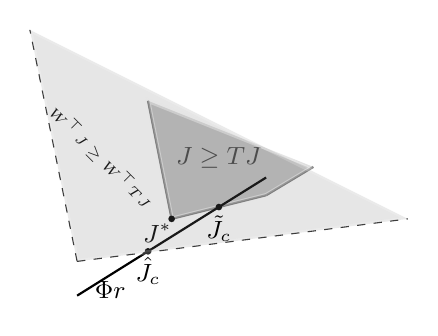
\begin{tikzpicture}[domain=-10:7.7,scale=0.6,font=\small,axis/.style={very thick, ->, >=stealth'}]
%\draw[line,thick,->] (-1,-0.625)--(4,-0.625);
%\draw[line,thick,->] (0,-1)--(0,4);
%\draw[line,thick,-](-0.2,-0.6)--(1,3);
\draw[line,thick,-](0.5,3.5)--(1,1);
\draw[line,thick,-](1,1)--(3,1.5);
\draw[line,thick,-](3,1.5)--(4,2.1);
\node[](one) at (2,2.3){\text{$J\geq TJ$}};
\node[rotate=-45](seven) at (-0.5,2.3){\text{\tiny $W^\top J\geq W^\top TJ$}};
\node[](two) at (-0.3,-0.5){\text{$\Phi r$}};
\node[](three) at (0.7,0.7){\text{$J^*$}};
%\draw[line,thick,-](0,0)--(4,2.5);
 \draw [ultra thick, draw=white, fill=gray, opacity=0.5]
       (0.5,3.5)--(1,1)--(3,1.5)--(4,2.1) -- cycle;
\draw[line,thick,-](-1,-0.625)--(3,1.8750);
 \fill (1,1)  circle[radius=2pt];
 \fill (2,1.25)  circle[radius=2pt];
 \fill (0.5,0.3125)  circle[radius=2pt];
\draw[line,dashed,-](-1,0.1)--(6,1);
\draw[line,dashed,-](-1,0.1)--(-2,5);
 \draw [ultra thick, draw=white, fill=gray, opacity=0.2]
       (-1,0.1)--(6,1)--(-2,5) -- cycle;
\node[] (four) at (2,0.8){\text{$\tilde{J}_c$}};
\node[] (six) at (0.5,-0.1){\text{$\hat{J}_c$}};
\end{tikzpicture}
%}
\caption{The outer lightly shaded region corresponds to GRLP constraints and the inner dark shaded region corresponds to the original constraints. The main contribution of the paper is to bound $||J^*-\hat{J}_c||$.}
\label{cartoon}
\end{figure}


\begin{figure}
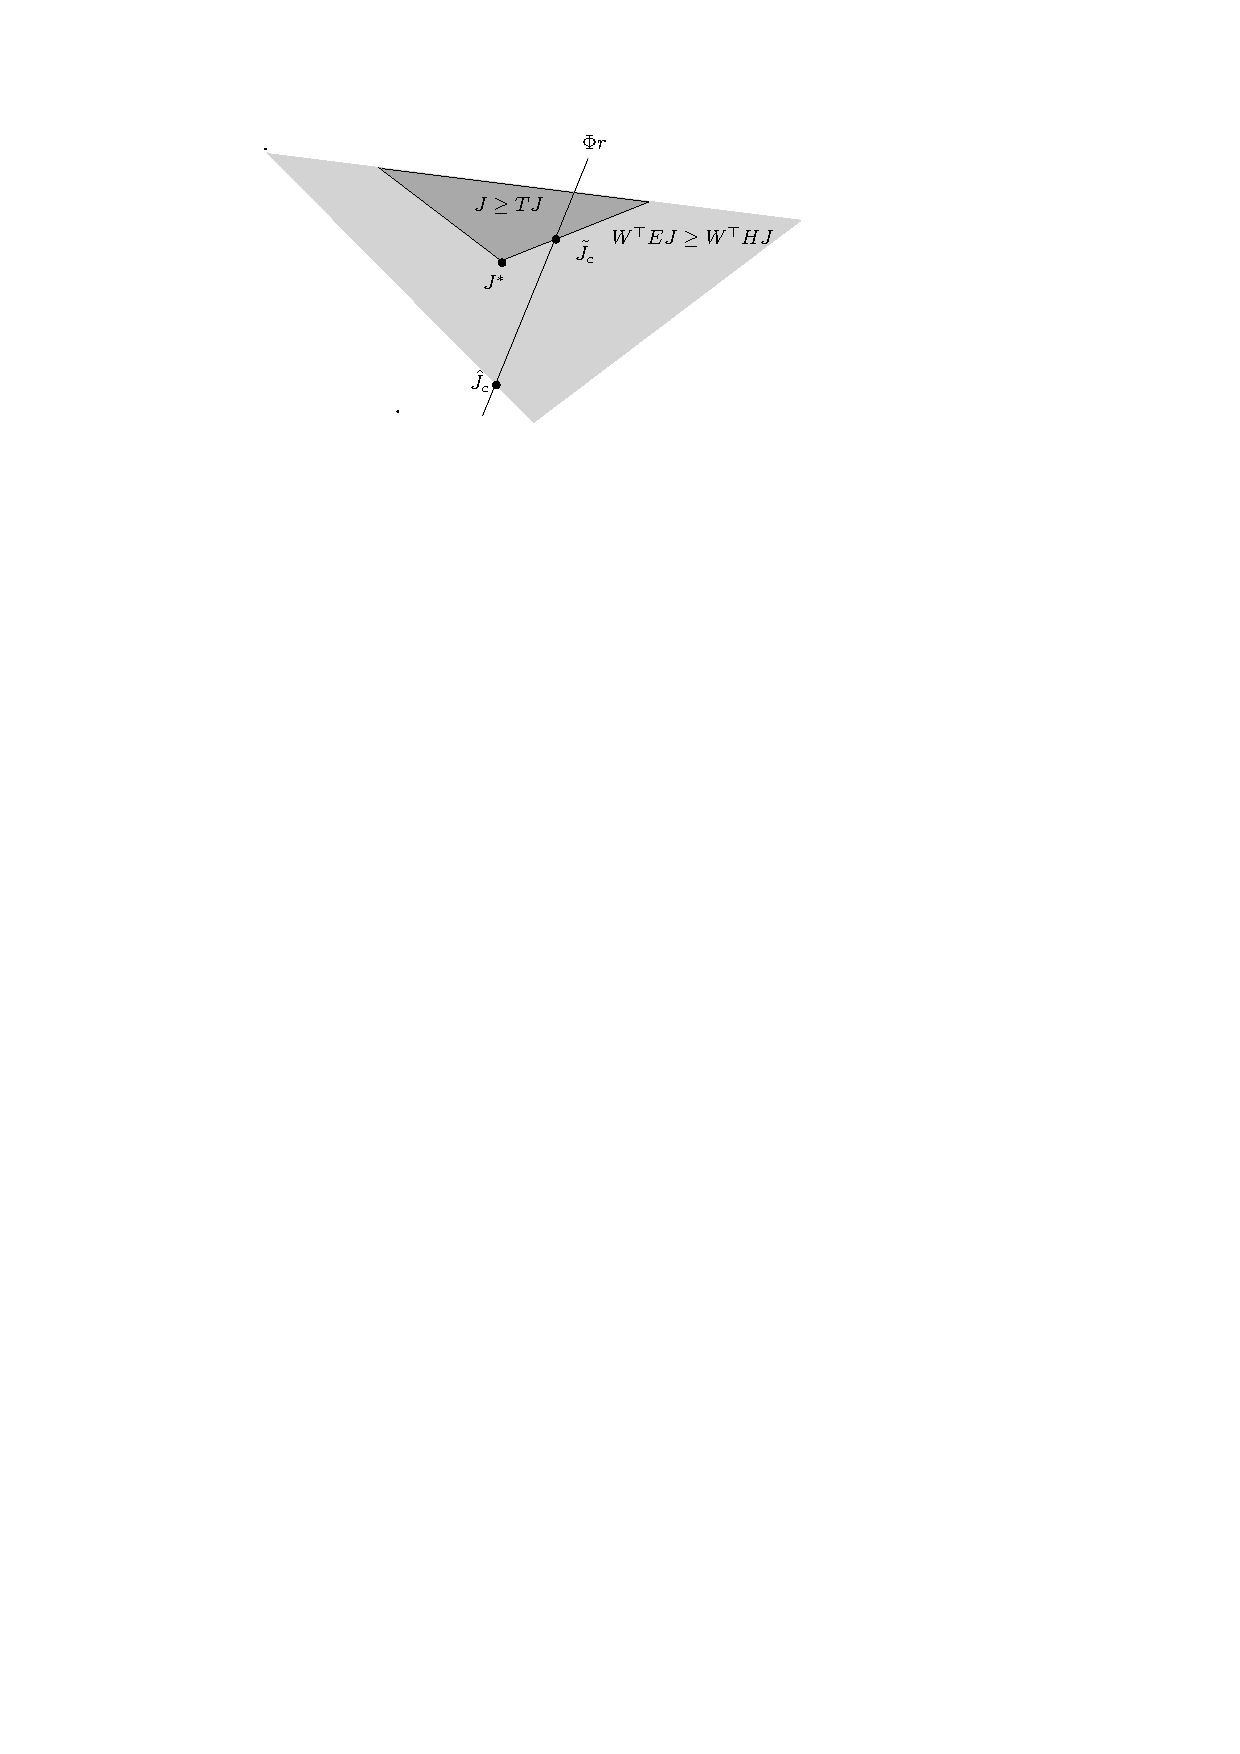
\includegraphics[scale=0.7]{cartoon_grlp.pdf}
\caption{
%\normalsize
The outer lightly shaded region corresponds to GRLP constraints and the inner dark shaded region corresponds to the original constraints. The main contribution of the paper is to bound $\norm{J^*-\hat{J}_c}$.}
\label{cartoon}
\end{figure}
\Cref{cartoon} shows the solutions to the LP, ALP and GRLP respectively. The error in ALP solution has already been studied in \cite{ALP}. Our objective is to study the extra source of error due to constraint approximation.
\section{Main Results}
In this section we present the main results of this paper in \Cref{cmt2} (we state improved bounds in \Cref{sec:improv}). Our bounds are expressed in terms of two novel contractions operators which we define in \Cref{lubpop,alubpop}. We now define two projection operators that are central to our error analysis and in them we assume that the set $\N'\subset \R^k$ is such that $\N' = \N + t \one$ for any $t\in \R$.
%The least upper bound (LUB) projection operator $\Gamma \colon \R^n \ra\R^n$ is defined below, see \eqref{gamdef}.
\begin{definition}\label{lubpop}
Given $J\in \R^n$ and the nonnegative valued vector $c\in \R^n_+$, define $r_{c,J}$ to be the solution to
\begin{align}
\label{lubplp}
\begin{split}
\underset{r\in \N'}{\min} &\,\, c^\top \Phi r\,\mb
\text{s.t.} \mb \Phi r\geq  TJ.
\end{split}
\end{align}
For $J\in \R^n$, $\Gamma J$, the \emph{least upper} (LU) projection of $J$ is defined as
\begin{align}\label{gamdef}
(\Gamma J)(i)\eqdef(\Phi r_{e_i,J})(i),\quad i=1,\ldots,n\,.
\end{align}
\end{definition}
The definition of the second operator is as follows:
\begin{definition}\label{alubpop}
Given $J\in \R^n$ and the nonnegative valued vector $c\in \R^n_+$, define $r'_{c,J}$ to be the solution to
\begin{align}\label{alubplp}
\underset{r\in \N'}{\min}& \,\mb c^\top \Phi r\,\mb
\text{s.t.} \,\,\, W^\top E \Phi r\geq W^\top HJ.
\end{align}
The \emph{approximate least upper} (ALU) projection operator
$\hg \colon \R^n \ra \R^n$ is defined as
\begin{align}\label{tgamdef}
(\hg J)(i)\eqdef(\Phi r'_{e_i,J})(i), \mb i=1,\ldots,n\,, J\in \R^n\,.
\end{align}
\end{definition}
\begin{remark}\label{ubrem}
To understand the meaning of $\Gamma$ (and $\hg$) define
\begin{align}\label{ubclass}
\F_J\eqdef\{\,\Phi r\,:\,\Phi r\geq TJ, r\in \N'\,\},
\end{align}
where $J\in \R^n$.
Disregarding the constraint $r\in \N'$,
$\F_J$ contains all vectors in the span of $\Phi$ that upper bound $TJ$. Further, since $(\Gamma J)(i) = \min\{ V(i) \,:\, V\in \F_J \}$, it also follows that $ V\ge \Gamma J $ holds for any $V\in \F_J$. Also $\Gamma J\geq T J$.\par
The operators $\Gamma$ and $\hg$ are closely related to ALP \eqref{alp} and GRLP \eqref{grlp} respectively and are only analytical tools that we will need to express our bounds and need not be computed in practice. It turns out that the novel operators ($\Gamma$ and $\hg$) are contraction maps (see \Cref{hgmaxcontramn}), a fact that is a key to our results (\Cref{cmt2mn,polthe}). At the outset we are interested in the candidate value functions in the constraint set $\N$ and want to study them using $\Gamma$ and $\hg$. However since the basis $\Phi$ contains $\one$ we make it helps our analysis to define the set $\N'$ in \Cref{lubplp,alubplp} to be `$\N$ plus its translations by $\one$'.
\end{remark}
%\subsection{Error Bounds}
\begin{theorem}[Error Bound for GRLP]
\label{cmt2}
Let $\one\in\R^k$ be in the column span of $\Phi$, then it holds that
\begin{enumerate}
\item The prediction error is bound as\\
$\norm{J^*-\hj}_{1,c}
\leq\frac{1}{1-\alpha}(6~\us{\min}{r\in \R^k}\norm{J^*-\Phi r}_{\infty}
+2\norm{\Gamma J^*-\hg J^*}_{\infty})$.
\item The control error is bound as\\
$\norm{J^* - J_{\hu}}_{1,c}
\leq 2\left(\frac{1}{(1-\alpha)^2}\right)\, \big( 2~\us{\min}{r\in \R^k} \norm{J^*-\Phi r}_{\infty}
+\norm{\Gamma J^*-\hg J^*}_{\infty}+\norm{\hj-\hg\hj}_{\infty}\big)$.
\end{enumerate}
\end{theorem}
\textbf{On Prediction Error:} The first factor in the right hand side of the prediction error in \Cref{cmt2} is related to the best possible approximation that can be achieved with the chosen feature matrix $\Phi$. This term is an carry over of the upper bound in ALP formulation as shown in \Cref{alpvanilla}. The second factor in the right hand side of the prediction error is related to constraint approximation and is completely defined in terms of $\Phi$, $W$ and $T$, and does not require knowledge of stationary distribution of the optimal policy.\par
\textbf{On Control Error:} The first two terms are quite similar to those in the bound for prediction error. The third term occurs due to the fact that $\Phi \geq T\Phi r$ that holds in the case of ALP does not hold in the case of GRLP.\par
\begin{comment}
\begin{theorem}[Control Error Bound in $\norm{\cdot}_{\infty}$]
\label{polthe}
Let $\hu$ be the greedy policy with respect to the solution $\hj$ of GRLP and $J_{\hu}$ be its value function.
% Let $r^*$ be as in Theorem~\ref{mt2mn}, then
Then,
\begin{align}\label{polthebnd}
\norm{J^* - J_{\hu}}_{1,c}
&\leq 2\left(\frac{c^\top \psi}{(1-\beta_{\psi})^2}\right)\, \big( 2\norm{J^*-\Phi r^*}_{\infty}
\nn\\&
+norm{\Gamma J^*-\hg J^*}_{\infty}+\norm{\hj-\hg\hj}_{\infty}\big).
\end{align}
\end{theorem}
\end{comment}
\begin{corollary}[Constraint Sampling]\label{st}
$W\in \{0,1\}^{nd\times m}$Let $s\in S$ be a state whose constraint is selected by $W$ (i.e., for some $i$ and all $(s',a)\in S\times A$,
$W_{s'a,i}=\delta_{s=s'}$.
Then
\begin{align*}%\label{sampexp}
|\Gamma J^*(s)-\hg J^*(s)|<|\Gamma J^*(s)-J^*(s)|.
\end{align*}
\end{corollary}
It is important to note that \Cref{rlpt} holds only in high probability and is valid only under idealized assumption of knowing the optimal policy $u^*$, while \Cref{cmt2} does not have these limitations.
In addition, the error $|\Gamma J^*(s) -\hg J^*(s)|$ (in \Cref{st} ) due to constraint approximation is less than the original projection error $|\Gamma J^*(s)-J^*(s)|$ due to function approximation. This means that for RLP to perform well it is important to retain the constraints corresponding to those states for which the linear function approximation via $\Phi$ is known to perform well.

\section{Least Upper Bound Projection}\label{sec:lubp}
The least upper bound (LUB) projection operator $\Gamma \colon \R^n \ra\R^n$ is defined as below:
\begin{definition}\label{lubpop}
Given $J\in \R^n$, its least upper bound projection is denoted by $\Gamma J$ and is defined as 
\begin{align}\label{gamdef}
(\Gamma J)(i)\stackrel{\Delta}{=}\underset{j=1,\ldots,k}{\min} (\Phi r_{e_j})(i), \mb \forall i=1,\ldots,n,
\end{align}
where $V(i)$ denotes the $i^{th}$ component of the vector $V\in \R^n$. Also in \eqref{gamdef}, $e_j$ is the vector with $1$ in the $j^{th}$ place and zeros elsewhere, and $r_{e_j}$ is a solution to the linear program in \eqref{lubplp} for $c=e_j$.
\begin{align}\label{lubplp}
r_c\stackrel{\Delta}{=}\min_{r\in \chi} &c^\top \Phi r,\nn\\
\text{s.t}\mb &\Phi r\geq  TJ.
\end{align}
\end{definition}
\begin{remark}
\begin{enumerate}
\item The definition of LUB operator $\Gamma \colon \R^n \ra \R^n$ involves $n$ associated linear programs.
\item Observe that $\Gamma J\geq TJ$ (follows from the fact that if $a\geq c$ and $b\geq c$, then $\min(a,b)\geq c$, where $a, b, c \in \R$).
\item Given $\Phi$ and $J\in \R^n$, define $\F\stackrel{\Delta}{=}\{\Phi r|\Phi r\geq TJ\}$. Thus $\F$ is the set of all vectors in the span of $\Phi$ that upper bound $TJ$. By fixing $c$ in the linear program in \eqref{lubplp} we select a unique vector $\Phi r_c \in \F$. The LUB projection operator $\Gamma$ picks $n$ vectors $\Phi r_{e_i},i=1,\ldots,n$ from the set $\F$ and $\Gamma J$ is obtained by computing their component-wise minimum.
\item Even though $\Gamma J$ does not belong to the span of $\Phi$, $\Gamma J$ collates the various best upper bounds that can be obtained via the linear program in \eqref{lubplp}.
\item The LUB operator $\Gamma$ in \eqref{gamdef} bears close similarity to the ALP in \eqref{alp}.
\end{enumerate}
\end{remark}
\begin{definition}\label{bestproj}
The LUB projection of $J^*$ is denoted by $\bj=\Gamma J^*$.
\end{definition}
We now characterize the LUB projection operator $\Gamma$ in the following lemmas (all the proofs are presented in the Appendix). As mentioned earlier, the error analysis depends on two $\max$-norm contraction operators the first of which is $\Gamma$. The important result of this section is Theorem~\ref{fxpres} and it relates the fixed point $\tilde{V}$ of $\Gamma$ to $J^*$.
\begin{lemma}\label{bestbnd}
Let $r^*\in \R^k$ be defined as $r^*\stackrel{\Delta}{=}\arg\min_{r\in R^k}||J^*-\Phi r||_\infty$, then 
\begin{align}
||J^*-\bj||_\infty\leq 2||J^*-\Phi r^*||_\infty.
\end{align}
\end{lemma}
\begin{proof}
The result follows from the definition of $\Gamma$ in \eqref{gamdef} and the construction of $V_0$, Assumption~\ref{one}, and the fact that $\Phi r^*+||J^*-\Phi r^*||_\infty \one\geq TJ^*$. To see this, note that
\begin{align}
&\Gamma J^*=\hj \geq J^*,\nn\\
&\Phi r^* +||J^*-\Phi r^*||_\infty\geq TJ^*= J^*.\nn\\
&\text{Thus,}\nn\\
&\Phi r^* +||J^*-\Phi r^*||_\infty\geq \Gamma J^*\geq TJ^*.
\end{align}
\end{proof}

\begin{lemma}\label{gmonotone}
For $J_1, J_2\in \R^n$ such that $J_1\geq J_2$, we have $\Gamma J_1\geq \Gamma J_2$.
\end{lemma}
\begin{proof}
Choose any $i\in \{1,\ldots,n\}$ and let $r^1_{e_i}$ and $r^2_{e_i}$ be solutions to the linear program in \eqref{lubplp} for $c=e_i$ with $J=J_1$ and $J=J_2$ respectively. Since $J_1\geq J_2$, we have $TJ_1\geq TJ_2$ and $e_i^\top \Phi r^1_{e_i} \geq e_i^\top \Phi r^2_{e_i}$, i.e., $(\Phi r^1_{e_i})(i)\geq (\Phi r^2_{e_i})(i)$. The result follows from the fact that $(\Gamma J)(i)=(\Phi r_{e_i})(i),\mb\forall J\in \R^n$, and our choice of $i$ was arbitrary.
\end{proof}
\begin{lemma}\label{lpsol}
Let $A\in \R^{u\times v}$, $b,c\in R^u$, $x_0 \in R^v$ and $b_0=Ax_0$. Then
\begin{align}
\min\{c^\top Ax:Ax\geq b+b_0\} =\min\{c^\top Ax:Ax\geq b\}+c^\top b_0.
\end{align}
\end{lemma}
\begin{proof}
The claim can be shown by a simple change of variables.
\end{proof}
\begin{lemma}\label{gshift}
Let $J_1\in \R^n$ and $t\in \R$ be a constant. If $J_2=J_1+k\one$, then $\Gamma J_2=\Gamma J_1+\alpha t\one$.
\end{lemma}
\begin{proof}
Consider the $i^{th}$ linear programs associated with $\Gamma J_1$ and $\Gamma J_2$. The result follows by using Lemma~\ref{lpsol} with $A=\Phi$, $b=TJ$, $c=e_i$, $b_0=\alpha t\mathbf{1}$ and $x_0=\alpha t e_i$.
\end{proof}
\begin{theorem}\label{gmaxcontra}
The operator $\Gamma  \colon \R^n\ra \R^n$ obeys the $\max$-norm contraction property with factor $\alpha$.
\end{theorem}
\begin{proof}
Given $J_1,J_2\in \R^n,$ let $\epsilon=||J_1-J_2||_\infty$. Thus,
\begin{align}\label{ineq}
J_2-\epsilon\one\leq J_1\leq J_2+\epsilon \one.
\end{align}
From Lemmas~\ref{gmonotone} and ~\ref{gshift}, we can write
\begin{align}\label{ineq}
\Gamma J_2-\alpha \epsilon\one\leq \Gamma J_1\leq \Gamma J_2+\alpha \epsilon\one.
\end{align}
\end{proof}
\begin{corollary}
The iterative scheme in \eqref{pvi} based on the LUB projection operator $\Gamma$ in \eqref{gamdef} converges to a unique fixed point $\tv$.
\begin{align}\label{pvi}
V_{n+1}&=\Gamma V_n,\mb \forall n\geq 0.
\end{align}
\end{corollary}
\begin{lemma}\label{gfp}
 $\tv$, the unique fixed point of the iterative scheme \eqref{pvi}, obeys $\tv\geq T\tv$.
\end{lemma}
\begin{proof}
Consider the $i^{th}$ linear program associated with $\Gamma \tv$. We know that $\Phi r_{e_i}\geq T \tv,\mb \forall i=1,\ldots, n$. The result follows from noting that $\tv$ is the unique fixed point of $\Gamma $ and that $\tv(i)=\underset{j=1,\ldots,n}{\min}(\Phi r_{e_j})(i)$.
\end{proof}
\begin{lemma}\label{relation1}
 $\tv$, the unique fixed point of the iterative scheme \eqref{pvi}, and the solution $\tj$ to the ALP in \eqref{alp}, obey the relation $\tj\geq\tv\geq J^*$.
\end{lemma}
\begin{proof}
Since $\tv\geq T\tv$ it follows that $\tv\geq J^*$. Let $\Phi r_1, \Phi r_2,\ldots,\Phi r_n$ be solutions to the ALP in \eqref{alp} for $c=e_1, e_2,\ldots,e_n$ respectively. Now consider the iterative scheme in \eqref{pvi} with $V_0(i)=\underset{j=1,\ldots, n}{\min}(\Phi r_j)(i)$. It is clear from the definition of $V_0$ that $\tj(i)\geq\Phi r_i(i)\geq V_0(i),\mb \forall i=1,\ldots,n$. Also from the monotone property of $T$, we have 
\begin{align}\label{lineq}
\Phi r_i&\geq V_0,\nn\\
T\Phi r_i&\geq T V_0,\mbox{we also have}\nn\\
\Phi r_i\geq T\Phi r_i&\geq T V_0,\mb\text{by taking component-wise minimum},\nn\\
V_0&\geq T V_0.
\end{align}
From the first three inequalitites in \eqref{lineq}, $\Phi r_i\geq T \Phi r_i\geq T V_0, \mb\forall i=1\to n$ and hence $V_0\geq TV_0$. Since $V_1=\Gamma V_0$, from the definition of $\Gamma$ in \eqref{gamdef} we have $V_0\geq V_1$, and recursively $V_{n}\geq V_{n+1}, \mb\forall n\geq 0$. So it follows that $\tj\geq V_0\geq V_1\ldots\geq \tv$.
\end{proof}
%!TEX root =  autocontgrlp.tex
Recall that $\bj = \Gamma J^*$.
\begin{theorem}\label{fxpres}
%Let $\tv$ be the fixed point of the iterative scheme in \eqref{pvi} and let $\bj$ be the best possible LUB projection of $J^*$ as in Definition~\ref{bestproj}. Then,
We have 
\begin{align}
||J^*-\tv||_\infty\leq \frac{1}{1-\alpha}||J^*-\bj||_\infty\,.
\end{align}
\end{theorem}
\begin{proof}
Recall that $\bj = \Gamma J^*$.
Now, by the triangle inequality and since $\Gamma$ is an $\alpha$-contraction,
\begin{align*}
\inorm{J^* - \tv } \le \inorm{ J^* - \Gamma J^* } + \inorm{\Gamma J^* - \Gamma \tv }
\le  \inorm{ J^* - \bj } + \alpha \inorm{J^* - \tv}\,.
\end{align*}
Solving the inequality gives the result.
\if0
Let $\epsilon=||J^*-\bj||_\infty$, and $\{V_n\},n\geq 0$ be the iterates of the scheme in \eqref{pvi} with $V_0=\bj$, then
\begin{align}
||J^*-\tv||_\infty&\leq ||J^*-V_0+V_0-V_1+V_1\ldots-\tv||_\infty\nn\\
&\leq ||J^*-V_0||_\infty+||V_0-V_1||_\infty+\ldots\nn
\end{align}
Since $||V_1-V_0||_\infty=||\Gamma \bj-\Gamma J^*||_\infty\leq\alpha||\bj-J^*||_\infty$, from Theorem~\ref{gmaxcontra},
\begin{align}
||J^*-\tv||_\infty&\leq \epsilon+\alpha\epsilon+\alpha^2\epsilon+\ldots\nn\\
&=\frac{\epsilon}{1-\alpha}.
\end{align}
\fi
\end{proof}


%!TEX root =  autocontgrlp.tex
\section{Approximate Least Upper Bound Projection}\label{sec:alubp}
We define an approximate least upper bound (ALUB) projection operator which has a structure similar to the GRLP and is an approximation to the LUB operator.
Recall that $W\in \R^{nd\times m}$ is the matrix in \eqref{grlp} which is assumed to satisfy Assumption~\ref{wassump}.
\begin{definition}\label{alubpop}
Given $J\in \R^n$ and the nonnegative valued vector $c\in \R^n_+$, define $r_{c,J}'$ to be the solution to 
\begin{align}\label{alubplp}
 \underset{r\in \R^k}{\min}& \,\mb c^\top \Phi r\,,\nn\\
 \text{s.t.}& \,\,\, W^\top E \Phi r\geq W^\top HJ\,,\qquad r \in \N\,.
\end{align}
Then, for $J\in \R^n$, $\hg J$, the approximate least upper bound (ALUB) projection of $J$ is defined as 
\begin{align}\label{tgamdef}
(\hg J)(i)\eqdef(\Phi \har_{e_i,J})(i), \mb i=1,\ldots,n\,.
\end{align}
\end{definition}
\noindent 
Note that under our assumptions on $\N$, $\hg$ is well-defined.
We now show that $\hg$ satisfies the monotone property and is linear along $[\one]$-rays with a factor smaller than one and hence it will follow that it is a contraction.
\begin{lemma}\label{tgmonotone}
For $J_1, J_2\in \R^n$ such that $J_1\leq J_2$, we have $\hg J_1\leq \hg J_2$.
\end{lemma}
\begin{proof}
By \cref{wassump}, $W^\top H: \R^n \to \R^m$ is monotone.
The proof then follows along the lines of Lemma~\ref{gmonotone}.
\end{proof}
\begin{lemma}\label{tgshift}
Let $J\in \R^n$ and $t\in \R$ be a constant. Then $\hg (J+t\one)=\hg J+\alpha t\one$.
\end{lemma}
\begin{proof}
The statement follows from Assumptions \ref{one}, \ref{wassump} and \ref{ass:n}, 
as well as Lemma~\ref{lpsol} using arguments along the lines of Lemma~\ref{gshift}. 
In particular, consider the $i^{th}$ linear program corresponding to $\hg J$ and $\hg (J+t\one)$. 
Now, the result follows by letting $A=W^\top E \Phi$, $b=W^\top H J$, 
$c=e_i$, $b_0=\alpha t \mathbf{1}$, 
$x_0=\alpha t e_1$,
noting that thanks to
\cref{one} and \ref{wassump}, $A x_0 = b_0$ and that thanks to
\cref{ass:n} \eqref{ass:n1}, $\N = \N + \alpha t e_1$.
\end{proof}
From these results, by~\cref{maxnorm} it immediately follows that $\hg$ is an $\alpha$-contraction with respect to the $\max$-norm:
\begin{theorem}\label{tgmaxcontra}
The operator $\hg \colon \R^n\ra \R^n$ obeys the $\max$-norm contraction property with factor $\alpha$.
\if0
 and the following iterative scheme based on the ALUB projection operator $\hg$, see \eqref{apvi}, converges to a unique fixed point $\hv$.
\begin{align}\label{apvi}
V_{n+1}&=\hg V_n,\mb n\geq 0.
\end{align}
\fi
\end{theorem}
\begin{proof}
As noted, this is immediate from \cref{tgmonotone,tgshift} and \cref{maxnorm}.
%Follows along similar lines as the proof of Theorem~\ref{gmaxcontra}.
\end{proof}
In what follows we denote by $\hv$ the unique fixed point of $\hg$:
\begin{align*}
\hv = \hg \hv\,.
\end{align*}
Recall that $\hj$ denotes the solution $\hj$ of the GRLP \eqref{grlp}. 
The vector $\hj$ dominates the vector $\hv$:
\begin{lemma}\label{relation2}
The vectors $\hv,\hj$ obey $\hj\geq\hv$.
\end{lemma}
\begin{proof}
The proof follows in a similar manner as the proof of Lemma~\ref{relation1}. To elaborate, let $\Phi r_1, \Phi r_2,\ldots,\Phi r_n$ be solutions to the GRLP in \eqref{grlp} for $c=e_1, e_2,\ldots,e_n$ respectively. Fix some other $c\in [0,1]^n$, $\sum_i c(i)=1$. Now consider the iterative scheme in \eqref{apvi} with $V_0(i)=\underset{j=1,\ldots,n}{\min}(\Phi r_j)(i)$.\par
We need to show $V_1\le V_0 \le \hj$ and then the desired result follows from Lemma~\ref{tgmonotone}. Since $(\Phi r_j)(i) \ge (\Phi r_i)(i)$ also holds for any $1\leq i,j\leq n$ we have $V_0(i)  = (\Phi r_i)(i)$. Also, since $\hj(i) \ge (\Phi r_i)(i),1\leq i \leq n$ it follows that $\hj\geq V_0$. Now, for showing that $V_1 \le V_0$ holds, fix any $i$. We need to show that $V_1(i)=(\hg V_0)(i) = (\Phi r_{e_i,V_0})(i) \leq V_0(i)$. By the definition of $r_{e_i,V_0}$ we know that $(\Phi r_{e_i,V_0})(i) \le (\Phi r)(i)$
holds for any $r$ such that $W^\top E \Phi r \ge W^\top H V_0$. Thus, it suffices to show that $r_i$ satisfies this latter inequality, i.e., $W^\top E \Phi r_i \ge W^\top H V_0$. For this, it clearly sufficient if $\Phi r_i \ge V_0$. This however directly follows from the definition of $V_0$.
\begin{comment}
It is clear from the definition of $V_0$ that $\hj(i),(\Phi r_j)(i)\geq(\Phi r_i)(i)$, $i=1,\ldots,n$.
In particular, it follows that $V_0(i) =( \Phi r_i)(i)$ and so
$\Phi r_i \geq V_0$.
From the monotone property of $T$ (viz. $H$) we have 
$H\Phi r_i\geq H V_0$ and also, by minimizing component-wise
$E\Phi r_i\geq H\Phi r_i\geq HV_0$. Thus,
$E V_0\geq H V_0$. 
\todoc[inline]{I lost why this was needed.
I think the proof would be much easier to understand if we introduced $r_{c,J} = \argmin_{r} \{ c^\top \Phi r \,:\, W^\top E \Phi r \ge W^\top H J\}$. We could start by saying we need $V_1\le V_0 \le \hj$ because then Lemma~\ref{tgmonotone} will give the desired result. Next, $V_0\le \hj$ holds because on the one hand, $\hj(i) \ge (\Phi r_i)(i)$ for any $i$, while on the other hand,
$(\Phi r_j)(i) \ge (\Phi r_i)(i)$ also holds for any $i,j$, hence $V_0(i)  = (\Phi r_i)(i)$. 
Now, for showing that $V_1 \le V_0$ holds, fix any $i$. We need to show that $(\hg V_0)(i) = \min_j (\Phi r_{e_j,V_0})(i) = (\Phi r_{e_i,V_0})(i)$ is less than $V_0(i)$. By the definition of $r_{e_j,V_0}$ we know that $(\Phi r_{e_i,V_0})(i) \le (\Phi r)(i)$
holds for any $r$ such that $W^\top E \Phi r \ge W^\top H V_0$. Thus, it suffices to show that $r_i$ satisfies this latter inequality,
i.e., $W^\top E \Phi r_i \ge W^\top H V_0$. For this, it clearly sufficient if $\Phi r_i \ge V_0$. This however directly follows 
from the definition of $V_0$.
}
Since $V_1=\hg V_0$, from the definition of $\hg$ in \eqref{gamdef} and the construction of $V_0$, we have $V_0\geq V_1$, and recursively $V_{n}\geq V_{n+1}, \mb n\geq 0$. So it follows that $\hj\geq V_0\geq V_1\ldots\geq \hv$.
\end{comment}
\end{proof}
The next result bounds the distance between $J^*$ and $\hv$ in terms of the distance of $\bj = \Gamma J^*$ and $J^*$, and that between $\bj$ and $\hg J^*$.
\begin{theorem}\label{mt1}
We have
\begin{align}
||J^*-\hv||_\infty\leq \frac{||J^*-\Gamma J^*||_\infty+||\Gamma J^*-\hg J^*||_\infty}{1-\alpha}.
\end{align}
\end{theorem}
\begin{proof}
By the triangle inequality,
\begin{align}
||J^*-\hv||\leq ||J^*-\hg J^*||+||\hg J^*-\hg \hv||\leq ||J^*-\hg J^*||+\alpha || J^*- \hv||
%||J^*-\hv||_\infty&\leq ||J^*-V_0+V_0-V_1+V_1\ldots-\hv||_\infty\nn\\
%&\leq ||J^*-V_0||_\infty+||V_0-V_1||_\infty+||V_1-V_2||_\infty+\ldots\nn\\
%&=||J^*-V_0||_\infty+||\hg J^*-\hg V_0||_\infty+\ldots\nn\\
%&\leq (\epsilon+\beta)+\alpha(\epsilon+\beta)+\ldots\nn\\
%&=\frac{\epsilon+\beta}{1-\alpha}
\end{align}
and so by reordering and another triangle inequality,
\begin{align*}
\norm{J^*-\hv}_{\infty} \le \frac{\norm{ J^*-\hg J^*}_{\infty}}{1-\alpha}
\le \frac{\norm{ J^*-\Gamma J^*}_{\infty}+\norm{\Gamma J^* - \hg J^*}_{\infty}}{1-\alpha}\,.
\end{align*}
\end{proof}
\noindent Combining this result with \cref{bestbnd} gives the following corollary:
\begin{corollary}\label{cmt1}
%Let $\hv$, $\bj$ be as in Theorem~\ref{mt1} and let $r^*\eqdef\argmin_{r\in \R^k}||J^*-\Phi r||_\infty$, then
We have
\begin{align}
||J^*-\hv||_\infty\leq \frac{2||J^*-\Phi r^*||_\infty+||\Gamma J^*-\hg J^*||_\infty}{1-\alpha}.
\end{align}
\end{corollary}
%\begin{proof}
%The result is obtained by using Lemma~\ref{bestbnd} to replace the term $||J^*-\bj||_\infty$ in Theorem~\ref{mt1}.
%\end{proof}

%!TEX root =  autocontgrlp.tex
\section{A simple bound}
The following lemmas relate the fixed point $\hv$ of $\hg$ to the solution $\hj$ of the GRLP in \eqref{grlp}.
\begin{lemma}\label{srw}
A vector
$\hat{r} \in \R^k$ is a solution to GRLP \eqref{grlp} iff it solves the following program:
\begin{align}\label{grlpeqprog}
\begin{split}
\min_{r\in \R^k}\, &||\Phi r-\hv||_{1,c}\\
\text{s.t.}\mb &\, W^\top E \Phi r\geq W^\top H \Phi r\,, \qquad r\in \N\,.
\end{split}
\end{align}
\end{lemma}
\begin{proof}
We know from Lemma~\ref{relation2} that $\hj = \Phi \hr \geq\hv$, and thus
the solutions to \eqref{grlp} do not change if we add the constraint $\Phi r \ge \hv$.
Now, under this constraint, minimizing $c^\top \Phi r$ is the same as
 minimizing 
\begin{align*}
||\Phi r-\hv||_{1,c}=\sum_{i=1}^n c(i) |(\Phi r)(i)-\hv(i)|=c^\top \Phi r-c^\top \hv\,.
\end{align*} 
\end{proof}
\begin{theorem}\label{mt2}
%Let $\hv$ be the solution to the iterative scheme in \eqref{apvi} and let $\hj=\Phi \hr$ be the solution to the GRLP. Let $\bj$ be the best possible approximation to $J^*$ as in Definition~\ref{bestproj}, and $||\Gamma J^* -\hg J^*||_\infty$ be the error due to ALUB projection and let $r^*\eqdef\underset{r\in \R^k}{\arg\min}||J^*-\Phi r||_\infty$, then
It holds that
\begin{align}
||\hj-\hv||_{1,c}\leq\frac{4||J^*-\Phi r^*||_\infty+||\Gamma J^*-\hg J^*||_\infty}{1-\alpha}.
\end{align}
\end{theorem}
\begin{proof}
Let $\gamma=||J^*-\Phi r^*||_\infty$. Then, since $T$ is an $\alpha$-contraction in the $\max$-norm,
$||J^*-T\Phi r^*||_\infty=||TJ^*-T\Phi r^*||_\infty\leq\alpha\gamma$ and hence by the triangle inequality,
\begin{align}\label{eq:tphir}
||T\Phi r^*-\Phi r^*||_\infty&\leq(1+\alpha)\gamma\,.
\end{align}
Let $r'= r^*+t e_1$ with $t>0$ to be chosen later.
Then, from \cref{one},
$T\Phi r' = T(\Phi r^* + t \one) = T \Phi r^* + \alpha t \one \le \Phi r^* + (\alpha t+ (1+\alpha) \gamma) \one$,
 where the inequality follows from~\eqref{eq:tphir}.
 Choosing $t$ so that $t = \alpha t+ (1+\alpha) \gamma$, or $t = \frac{(1+\alpha)\gamma}{1-\alpha}$, we get
 that $T\Phi r' \le \Phi r'$. Hence, $r'$ is feasible to the ALP \eqref{alp} and 
since, thanks to \cref{wassump}, 
any feasible solution to \eqref{alp} is also a feasible solution to the GRLP  \eqref{grlp},
$r'$ is also feasible to \eqref{grlp}. Thus, 
\begin{align}
||\hj-\hv||_{1,c}&\leq||\Phi r'-\hv||_{1,c}\nn &(\text{thanks to Lemma~\ref{srw}}) \\ %\vspace{10pt}
&\leq||\Phi r'-\hv||_\infty\mb & (\text{since $c$ is a distribution})\nn\\
&\leq||\Phi r'-J^*||_\infty+||J^*-\hv||_\infty\,. & (\text{triangle inequality}) \label{mt2eq0}
\end{align}
Now, by another triangle inequality,
\begin{align}
||\Phi r'-J^*||_\infty&\leq ||\Phi r^* -J^*||_\infty+||\Phi r'-\Phi r^*||_\infty
\leq \gamma+\frac{(1+\alpha)\gamma}{1-\alpha}=\frac{2\gamma}{1-\alpha}.
\label{mt2eq1}
\end{align}
The result follows by combining this bound with \eqref{mt2eq0} and Corollary~\ref{cmt1}.
\end{proof}

\begin{corollary}[Prediction error bound]
\label{cmt2}
%Let $\hj$, $\hv$, $r^*$ and $J^*$ be as in Theorem~\ref{mt2}, then \todoc{Where is the effect of $\chi$?}
We have
\begin{align}\label{finalbnd}
||J^*-\hj||_{1,c}\leq\frac{6 ||J^*-\Phi r^*||_\infty+2||\Gamma J^*-\hg J^*||_\infty}{1-\alpha}\,.
\end{align}
\end{corollary}
\begin{proof}
We have
$
||J^*-\hj||_{1,c}\leq||J^*-\hv||_{1,c}+||\hv-\hj||_{1,c}
\leq||J^*-\hv||_\infty+||\hv-\hj||_{1,c}
$.
The result now follows from Corollary~\ref{cmt1} and Theorem~\ref{mt2}.
\end{proof}
The results presented in Corollary~\ref{cmt2} is in the $L_\infty$-norm. In the next section, we make use of Lyapunov functions to provide an improved bound in the weighted $L_\infty$-norm.

\section{Improved Bounds}\label{sec:improv}
In this section, we present improved error bounds by making use of Lyapunov functions. 
\begin{lemma}\label{bestbndmn}
Let $r^*\in \R^k$ be defined as $r^*\stackrel{\Delta}{=}\arg\min_{r\in R^k}||J^*-\Phi r||_{\infty,1/\psi}$, then 
\begin{align}
||J^*-\bj||_{\infty,1/\psi}\leq 2||J^*-\Phi r^*||_{\infty,1/\psi}.
\end{align}
\end{lemma}
\begin{proof}
The result follows from the definition of $\Gamma$ in \eqref{gamdef}, Assumption~\ref{lyap} and the fact that $\Phi r^*+||J^*-\Phi r^*||_{\infty,1/\psi} \psi\geq TJ^*$.
\end{proof}

Since most of our analysis in sections~\ref{sec:lubp} and ~\ref{sec:alubp} depended on showing that $\Gamma$ is a contraction map in the $L_\infty$ norm we first show that $\Gamma$ is also a contraction map in the modified $L_\infty$ norm.
\begin{lemma}\label{gshiftmn}
Let $J_1\in \R^n$ and $k\in \R$ be a constant. If $J_2=J_1+k\psi$, then $\Gamma J_2\leq \Gamma J_1+\beta_{\psi} k\psi$.
\end{lemma}
\begin{proof}
The result follows in a similar manner as the proofs for Lemmas~\ref{gshift} and ~\ref{tgshift} by using the result in Lemma~\ref{lpsol}.
\end{proof}
\begin{theorem}\label{gmaxcontramn}
The operator $\Gamma  \colon \R^n\ra \R^n$ is a contraction operator in modified $L_\infty$ with factor $\beta_{\psi}$.
\end{theorem}
\begin{proof}
Given $J_1,J_2\in \R^n$ let $\epsilon=||J_1-J_2||_{\infty,1/\psi}$. Thus
\begin{align}\label{ineq}
J_2-\epsilon\psi\leq J_1\leq J_2+\epsilon \psi.
\end{align}
From Lemmas~\ref{gmonotone} and ~\ref{gshiftmn}, we can write
\begin{align}\label{ineq}
\Gamma J_2-\beta_{\psi} \epsilon\psi\leq \Gamma J_1\leq \Gamma J_2+\beta_{\psi} \epsilon\psi.
\end{align}
Thus
\begin{align}
||\Gamma J_1-\Gamma J_2||_{\infty,1/\psi}\leq \beta_{\psi} ||J_1-J_2||_{\infty,1/\psi}.
\end{align}
\end{proof}
\begin{corollary}\label{hgmaxcontramn}
$\hg$ is also a contraction map in the modified $L_\infty$ norm.
\end{corollary}
\begin{proof}
Follows from arguments similar to Theorem~\ref{gmaxcontramn}.
\end{proof}
\begin{lemma}\label{cmt1mn}
Let $\hv$, $\bj$ be as in Theorem~\ref{mt1} and let $r^*\stackrel{\Delta}{=}\arg\min_{r\in \R^k}||J^*-\Phi r||_{\infty,1/\psi}$ then
\begin{align}
||J^*-\hv||_{\infty,1/\psi}\leq \frac{2||J^*-\Phi r^*||_{\infty,1/\psi}+||\Gamma J^*-\hg J^*||_{\infty,1/\psi}}{1-\beta_{\psi}}.
\end{align}
\end{lemma}
\begin{proof}
The proof follows from Lemma~\ref{gmaxcontramn}, Corollary~\ref{hgmaxcontramn} and by replacing the $||\cdot||_\infty$ norm by $||\cdot||_{\infty,1/\psi}$ in the arguments presented in sections~\ref{sec:lubp} and ~\ref{sec:alubp} leading to Corollary~\ref{cmt1}.
\end{proof}\\
We now recall Lemma~$4.3$ of \cite{ALP}.
\begin{lemma}\label{restate}
Let $\psi$ be a Lyapunov function that belongs to the column span of $\Phi$ , $r \in \R^k$ be an arbitrary vector and let $r'$ be such that
\begin{align}
\Phi r'=\Phi r+||J^*-\Phi r||_{\mn}(\frac{1+\beta_{\psi}}{1-\beta_{\psi}})\psi.
\end{align}
Then $r'$ is feasible for the ALP in \eqref{alp}.
\end{lemma}
\begin{theorem}\label{mt2mn}
Let $\hv$ be the solution to the iterative scheme in \eqref{apvi} and let $\hj=\Phi \hr$ be the solution to the GRLP. Let $\bj$ be the best possible approximation to $J^*$ as in Definition~\ref{bestproj}, and $||\Gamma J^* -\hg J^*||_{\infty,1/\psi}$ be the error due to ALUB projection and let $r^*\stackrel{\Delta}{=}\underset{r\in \R^k}{\arg\min}||J^*-\Phi r||_{\infty,1/\psi}$, then
\begin{align}
||\hj-\hv||_{1,c}&\leq \frac{c^\top \psi}{1-\beta_\psi}(4||J^*-\Phi r^*||_{\mn}
%\nn\\&
+||\Gamma J^*-\hg J^*||_{\mn}).
\end{align}
\end{theorem}
\begin{proof}
Let $\gamma=||J^*-\Phi r^*||_{\infty,1/\psi}$, then by choosing $r'$ as in Lemma~\ref{restate} we have
\begin{align}
||\Phi r'-J^*||_{\mn}&\leq ||\Phi r^*-J^*||_{\mn}+||\Phi r'-\Phi r^*||_{\mn}\nn\\
&=\gamma+\frac{1+\beta_\psi}{1-\beta_\psi}\gamma\nn\\
&=\frac{2}{1-\beta_\psi}\gamma.\nn
\end{align}
Since $r'$ is also feasible for the GRLP in \eqref{grlp} we have
\begin{align}
||\hj-\hv||_{1,c}&\leq||\Phi r'-\hv||_{1,c}\nn\\
&=\sum_{s\in S}c(s)\psi(s)\frac{|\Phi r'(s)-\hv(s)|}{\psi(s)}\nn\\
&\leq c^\top \psi ||\Phi r'-\hv||_{\infty,1/\psi}\nn\\
&\leq c^\top \psi (||\Phi r'-J^*||_{\infty,1/\psi}+||J^*-\hv||_{\infty,1/\psi}).
\end{align}
The result follows from Corollary~\ref{cmt1}.\\
\textbf{Main Result~$1$: Prediction Error bound in modified $L_\infty$-norm}
\end{proof}
\begin{theorem}\label{cmt2mn}
Let $\hj$, $\hv$, $r^*$ and $J^*$ be as in Theorem~\ref{mt2mn}, then
\begin{align}\label{finalbndmn}
||J^*-\hj||_{1,c}&\leq\frac{c^\top\psi}{1-\beta_\psi}(6 ||J^*-\Phi r^*||_{\mn}
%\nn\\&
+2||\Gamma J^*-\hg J^*||_{\mn}).
\end{align}
\end{theorem}
\begin{proof}
\begin{align}
||J^*-\hj||_{1,c}&\leq||J^*-\hv||_{1,c}+||\hv-\hj||_{1,c}\nn\\
&\leq c^\top \psi ||J^*-\hv||_{\mn}+||\hv-\hj||_{1,c}.\nn
\end{align}
The result now follows from Lemma~\ref{cmt1mn} and Theorem~\ref{mt2mn}.
\end{proof}\\


\textbf{Main Result $2$: Control Error bound in modified $L_\infty$-norm}\\
We now bound the performance of the greedy policy $\hu$.
\begin{theorem}\label{polthe}
Let $\hu$ be the greedy policy with respect to the solution $\hj$ of the GRLP and $J_{\hu}$ be its value function. Let $r^*$ be as in Theorem~\ref{mt2mn}, then
\begin{align}\label{polthebnd}
||J_{\hu}-\hj||_{1,c}&\leq 2\big(\frac{c^\top \psi}{1-\beta_{\psi}}\big)^2 \big(6 ||J^*-\Phi r^*||_{\mn}
%\nn\\&
+2||\Gamma J^*-\hg J^*||_{\mn}\big).
\end{align}
\end{theorem}
\begin{proof}
\begin{align}\label{polderv}
||J_{\hu}-\hj||_{1,c}&=||(I-\alpha P_{\hu})^{-1}(T\hj-\hj)||_{1,c}\nn\\
&\leq c^\top(I-\alpha P_{\hu})^{-1}|T\hj-\hj|\nn\\
&\leq c^\top (I-\alpha P_{\hu})^{-1} \psi ||T\hj-\hj||_{\mn}\nn\\
&\leq \frac{c^\top \psi}{1-\beta_{\psi}}||T\hj-\hj||_{\mn}\nn\\
&\leq \frac{c^\top \psi}{1-\beta_{\psi}}||T\hj-TJ^* +J^*- \hj||_{\mn}\nn\\
&\leq \frac{c^\top \psi}{1-\beta_{\psi}}(||T\hj-TJ^*||_{\mn} +||J^*- \hj||_{\mn})\nn\\
&\leq \frac{c^\top \psi}{1-\beta_{\psi}}(1+\beta_{\psi})||J^*- \hj||_{\mn},
\end{align}
where in the second inequality, for $x=(x_1,\ldots,x_n)^\top\in \R^n$, $|x|=(|x_1|,\ldots,|x_n|)^\top\in \R^n$. Now
\begin{align}
||J^*-J_{\hu}||_{1,c}&\leq ||J^*-\hj||_{1,c}+||J_{\hu}-\hj||_{1,c}\nn\\
&\leq c^\top \psi ||J^*-\hj||_{\mn}+c^\top \psi\frac{1+\beta_\psi}{1-\beta_\psi}||J^*- \hj||_{\mn}\nn\\
&=\frac{2c^\top \psi}{1-\beta_{\psi}}||J^*- \hj||_{\mn}.
\end{align}
The result now follows by substituting the value of $||J^*- \hj||_{\mn}$ from Corollary~\ref{cmt2mn}.
\end{proof}
\begin{note}
By letting $\etmn=||\Gamma J^*-J^*+J^*-\hg J^*||_{\mn}\leq 2||J^*-\Phi r^*||_{\infty,1/\psi}+||J^*-\hg J^*||_{\mn}$ (inequality follows from Lemma~\ref{bestbndmn}), we can also modifiy the bounds in \eqref{finalbnd} and \eqref{polthe} as
\begin{align}
\label{loose1}||J^*-\hj||_{1,c}&\leq\frac{c^\top\psi}{1-\beta_\psi}(10 ||J^*-\Phi r^*||_{\mn}
%\nn\\&
+2||J^*-\hg J^*||_{\mn}).\\
\label{loose2}||J_{\hu}-\hj||_{1,c}&\leq 2\big(\frac{c^\top \psi}{1-\beta_{\psi}}\big)^2 \big(10 ||J^*-\Phi r^*||_{\mn}
%\nn\\&
+2||J^*-\hg J^*||_{\mn}\big).
\end{align}
Here the term $||J^*-\hg J^*||$ in \eqref{loose1} and \eqref{loose2} captures the error due to the use of both $\Phi$ and $W$. Though, \eqref{loose1} and \eqref{loose2} might be loser bounds than \eqref{finalbndmn} and \eqref{polthebnd} respectively, the aim here is to capture the error due to function approximation as well as constraint reduction in a single term.
\end{note}


%!TEX root =  autocontgrlp.tex
\subsection{Discussion}
\begin{comment}
The error bounds in the main results (Theorems~\ref{cmt2mn} and \ref{polthe}) contain two factors, namely
\begin{enumerate}
\item $\min_{r\in \R^k} ||J^*-\Phi r||_{\mn}$, and
\item $||\Gamma J^*-\hg J^*||_{\mn}$.
\end{enumerate}
The first factor is related to the best possible approximation that can be achieved with the chosen feature matrix $\Phi$. This term is inherent to the ALP formulation and it appears in the bounds provided by \cite{ALP}.\par
The second factor is related to constraint approximation and is completely defined in terms of $\Phi$, $W$ and $T$, and does not require knowledge of stationary distribution of the optimal policy. It makes intuitive sense since given that $\Phi$ approximates $J^*$, it is enough for $W$ to depend on $\Phi$ and $T$ without any additional requirements.\par An interesting feature is that unlike prior work on constraint sampling based on concentration inequalities (e.g.,  \cite{CS}), our analysis is based on contraction operators and is completely deterministic.
In particular, the error term $\etmn$ gives new insights into constraint selection:
\begin{theorem}\label{st}
Let $s\in S$ be a state whose constraint is selected by $W$ (i.e., for some $i$ and all $(s',a)\in S\times A$, 
$W_{s'a,i}=\delta_{s=s'}$. 
Then
\begin{align}\label{sampexp}
|\Gamma J^*(s)-\hg J^*(s)|<|\Gamma J^*(s)-J^*(s)|.
\end{align}
\end{theorem}
\end{comment}
\begin{proof}
Let $r_{e_s,J^*}$ and ${r}'_{e_s,J^*}$ be solutions to the linear programs in \eqref{lubplp} and \eqref{alubplp} respectively for $c=e_s$ and $J=J^*$. It is easy to note that $r_{e_s,J^*}$ is feasible for the linear program in \eqref{alubplp} for $c=e_s$ and $J^*$, and hence it follows that $(\Phi r_{e_s,J^*})(s)\geq (\Phi {r}'_{e_s,J^*})(s)$. However, since the constraints with respect to state $s$ have been chosen we know that $(\Phi {r}'_{e_s,J^*})(s)\geq J^*(s)$. The proof follows from noting that $(\Gamma J^*)(s)=(\Phi r_{e_s,J^*})(s)$ and $\hg J^*(s)=(\Phi {r}_{e_s,J^*})(s)$.
\end{proof}
\begin{comment}
The expression in \eqref{sampexp} in Theorem~\ref{st} says that the additional error $|\Gamma J^*(s) -\hg J^*(s)|$ due to constraint approximation is less than the original projection error $|\Gamma J^*(s)-J^*(s)|$ due to function approximation. This means that for the RLP to perform well it is enough to retain those states for which the linear function approximation via $\Phi$ is known to perform well. The modified $L_\infty$ norm in \eqref{finalbndmn} comes to our rescue to control the error due to those states that are not chosen.
\end{comment}

\section{Conclusion}
The approximate linear programming (ALP) is a widely employed method to handle MDPs with large number of states. However, an important shortcoming of the ALP is that it has large number of constraints, which is tackled in practice by sampling a tractable number of constraints from the ALP to formulate and solve a reduced linear program (RLP). The RLP has been found to work well empirically in various domains ranging from queues to Tetris games, and performance guarantees are for a specific RLP formulated under idealized assumptions. Alternatively, function approximation in the dual variables of the ALP has been another approach that has been employed in literature \cite{ALP-Bor,dolgov} to address the issue of large number of constraints. However \cite{ALP-Bor,dolgov} do not provide theoretical characterization for the function approximation of the dual variables.\par
In this paper, we introduced a novel framework based on the generalized reduced linear program formulation to study constraint reduction. The constraints of the GRLP were obtained as positive linear combinations of the original ALP. We provided an error bound that relates the optimal value function to the solution of the GRLP. Our error bound contained two terms, one inherent to the ALP formulation and the other due to constraint reduction. We also made qualitative and quantitative observations about the nature of the error term that arose due to constraint reduction. Our analysis also revealed the fact that it is not always necessary to sample according to the stationary distribution of the optimal policy and, in fact, potentially several different constraint sampling/approximation strategies might work. In particular, we also theoretically justified linear function approximation of the constraints. We also discussed the results and provided a numerical example in the domain of controlled queues. To conclude, we observe that by providing a novel theoretical framework to study constraint approximation, this paper provides important results that add to the theory of ALP.



%\input{example}
%\input{discussion}
\bibliographystyle{plain}
\bibliography{ref.bib}
\newpage
\onecolumn
%\begin{appendix}
\textbf{On choice of $\N$:}\\
It is desirable to get rid of the assumption that $\tr\in \N$ without affecting our arguments. Note that the set $\N$ is not used in ALP \eqref{alp} and the feasible set of ALP can be specified as the set $\S\eqdef\{r\in \R^k| \Phi r \geq T\Phi r\}$. Further, the only property about $\S$ that we used in our argument (\Cref{restate}) was that $r'= r^*+\norm{J^*-\Phi r^*}_{\mn} \left(\frac{1+\beta_{\psi}}{1-\beta_{\psi}}\right)\, r_0 \in \S$. Thus, so long as $\N$ contains $r'$ it is not necessary for it to contain $\tr$.\par
Let $g_{\min}=\underset{a,s}{\min}g_a(s)$, $g_{\max}=\underset{a,s}{\max}g_a(s)$ and define $r^*\eqdef\underset{r\in \R^k}{\arg\min}\norm{J^*-\Phi r}_{\mn}$. Now $\frac{g_{\min}}{1-\alpha}\leq J^* \leq \frac{g_{\max}}{1-\alpha}$ and since $\mathbf{1}$ is in the basis, we have $\norm{J^*-\Phi r^*}_{\mn}\leq \frac{g_{\max}-g_{\min}}{1-\alpha}$ (making use of the fact that for any sensible choice of Lyapunov function $\norm{J^*-\Phi r^*}_{\mn}\leq \norm{J^*-\Phi r^*}_{\infty}$).  The fact that $r'\in \N$ can then be ensured when $\N\eqdef\{\r| a\leq \Phi r\leq b\}$, where $a=\frac{g_{\min}}{1-\alpha}$ and $b=\frac{g_{\max}}{1-\alpha}+\frac{1+\beta_{\psi}}{1-\beta_{\psi}}\frac{g_{\max}-g_{\min}}{1-\alpha}$.
\end{appendix}

\end{document}
